\documentclass[12pt]{article}
\usepackage{amsmath, amssymb, amsthm}
\usepackage{geometry}
\usepackage{array}
\usepackage{enumitem}
\usepackage{titlesec}
\usepackage[dvipsnames, table]{xcolor}
\usepackage{fancyhdr}
\usepackage{tcolorbox}
\usepackage{microtype}
\usepackage{multicol}
\usepackage{booktabs}
\usepackage{multirow}
\usepackage{titletoc}
\usepackage{tabularx}
\usepackage{tikz}
\usetikzlibrary{calc, arrows.meta, decorations.pathreplacing}

\makeatletter
\newcommand\needspace[1]{%
  \begingroup\setlength\dimen@{#1}%
  \vskip\z@\@plus\dimen@\penalty -200%
  \vskip\z@\@plus-\dimen@\vskip\dimen@\penalty 9999%
  \vskip-\dimen@\vskip\z@skip\endgroup}
\makeatother

\tcbuselibrary{skins, breakable}
\geometry{margin=0.85in, top=1in, bottom=1in, headheight=15pt}

%-- Colours
\definecolor{primary}  {RGB}{27,  79, 114}
\definecolor{accent}   {RGB}{46, 134, 193}
\definecolor{lightbg}  {RGB}{234,244,251}
\definecolor{tealclr}  {RGB}{0,  110,  90}
\definecolor{tealbg}   {RGB}{220,245,240}
\definecolor{amberclr} {RGB}{160, 90,   0}
\definecolor{amberbg}  {RGB}{255,243,220}
\definecolor{purpleclr}{RGB}{90,  20, 140}
\definecolor{purplebg} {RGB}{240,228,255}
\definecolor{redclr}   {RGB}{150,  20,  20}
\definecolor{redbg}    {RGB}{255,228,228}
\definecolor{greenclr} {RGB}{20, 120,  40}
\definecolor{greenbg}  {RGB}{220,248,228}
\definecolor{grayclr}  {RGB}{80,  80,  80}
\definecolor{graybg}   {RGB}{245,245,245}
\definecolor{darktext} {RGB}{44,  62,  80}
\definecolor{gold}     {RGB}{183,149, 11}
\definecolor{goldbg}   {RGB}{254,249,231}
\definecolor{cardred}  {RGB}{192,  0,   0}

%-- Card macro
\newcommand{\mcard}[3]{%
  \tikz[baseline=-1pt]{
    \draw[rounded corners=2pt,fill=white,draw=gray!55,line width=0.5pt](0,0)rectangle(0.58,0.82);
    \node[font=\fontsize{6}{7}\selectfont\bfseries,text=#3]at(0.12,0.69){#1};
    \node[font=\fontsize{12}{13}\selectfont,text=#3]at(0.29,0.37){#2};
    \node[font=\fontsize{6}{7}\selectfont\bfseries,text=#3,rotate=180]at(0.46,0.13){#1};}%
}
\newcommand{\HS}{\textcolor{cardred}{$\heartsuit$}}
\newcommand{\DS}{\textcolor{cardred}{$\diamondsuit$}}
\newcommand{\SPS}{$\spadesuit$}
\newcommand{\CS}{$\clubsuit$}

%-- TOC
\setcounter{secnumdepth}{0}\setcounter{tocdepth}{1}
\renewcommand{\contentsname}{}
\titlecontents{section}[18pt]{\addvspace{5pt}\bfseries\color{primary}}{}{}
  {\color{accent!60}\titlerule*[5pt]{.}\textbf{\color{accent}\contentspage}}

%-- Page style
\pagestyle{fancy}\fancyhf{}
\fancyhead[L]{\small\color{primary}\textbf{Statistical Inference}\;\textcolor{accent}{|}\;Complete Workbook}
\fancyhead[R]{\small\color{darktext}BS-IV Mathematics}
\renewcommand{\headrulewidth}{0pt}
\fancyhead[C]{\color{accent}\rule[-1ex]{\textwidth}{1.2pt}}
\fancyfoot[C]{\small\color{darktext}\thepage}

%-- Section headings
\titleformat{\section}{\needspace{8\baselineskip}\large\bfseries\color{primary}}{}{0em}{}
  [\color{accent}\rule{\linewidth}{2pt}]
\titlespacing*{\section}{0pt}{18pt}{8pt}
\titleformat{\subsection}{\needspace{5\baselineskip}\normalsize\bfseries\color{accent}}{}{0em}{}
\titlespacing*{\subsection}{0pt}{10pt}{3pt}
\titleformat{\subsubsection}{\needspace{3\baselineskip}\small\bfseries\color{tealclr}}{}{0em}{}
\titlespacing*{\subsubsection}{0pt}{8pt}{2pt}

%-- tcolorbox environments
\newtcolorbox{defbox}[1][]{enhanced,arc=4pt,boxrule=1.5pt,
  colback=tealbg,colframe=tealclr,left=10pt,right=10pt,top=7pt,bottom=7pt,
  title={\small\bfseries\color{white}Definition\ifx&#1&\else\ ---\ #1\fi},colbacktitle=tealclr,
  attach boxed title to top left={xshift=10pt,yshift=-\tcboxedtitleheight/2},
  boxed title style={arc=3pt,colframe=tealclr,boxrule=0pt}}

\newtcolorbox{thmbox}[1][]{enhanced,arc=4pt,boxrule=1.5pt,
  colback=amberbg,colframe=amberclr,left=10pt,right=10pt,top=7pt,bottom=7pt,
  title={\small\bfseries\color{white}Theorem\ifx&#1&\else\ ---\ #1\fi},colbacktitle=amberclr,
  attach boxed title to top left={xshift=10pt,yshift=-\tcboxedtitleheight/2},
  boxed title style={arc=3pt,colframe=amberclr,boxrule=0pt}}

\newtcolorbox{examplebox}[1][]{enhanced,breakable,arc=4pt,boxrule=1.5pt,
  colback=white,colframe=amberclr,left=10pt,right=10pt,top=7pt,bottom=7pt,
  title={\small\bfseries\color{white}#1},colbacktitle=amberclr,
  attach boxed title to top left={xshift=10pt,yshift=-\tcboxedtitleheight/2},
  boxed title style={arc=3pt,colframe=amberclr,boxrule=0pt}}

\newtcolorbox{derivbox}[1][]{enhanced,breakable,arc=4pt,boxrule=1.5pt,
  colback=lightbg,colframe=primary,left=10pt,right=10pt,top=7pt,bottom=7pt,
  title={\small\bfseries\color{white}Derivation\ifx&#1&\else\ ---\ #1\fi},colbacktitle=primary,
  attach boxed title to top left={xshift=10pt,yshift=-\tcboxedtitleheight/2},
  boxed title style={arc=3pt,colframe=primary,boxrule=0pt}}

\newtcolorbox{formulabox}[1][]{enhanced,arc=4pt,boxrule=1.5pt,
  colback=lightbg,colframe=primary,left=10pt,right=10pt,top=7pt,bottom=7pt,
  title={\small\bfseries\color{white}Formula\ifx&#1&\else\ ---\ #1\fi},colbacktitle=primary,
  attach boxed title to top left={xshift=10pt,yshift=-\tcboxedtitleheight/2},
  boxed title style={arc=3pt,colframe=primary,boxrule=0pt}}

\newtcolorbox{histbox}{enhanced,arc=4pt,boxrule=1.5pt,
  colback=graybg,colframe=grayclr,left=10pt,right=10pt,top=7pt,bottom=7pt,
  title={\small\bfseries\color{white}Historical Background},colbacktitle=grayclr,
  attach boxed title to top left={xshift=10pt,yshift=-\tcboxedtitleheight/2},
  boxed title style={arc=3pt,colframe=grayclr,boxrule=0pt}}

\newtcolorbox{keybox}{enhanced,borderline west={4pt}{0pt}{purpleclr},
  colback=purplebg!55,colframe=white,arc=0pt,boxrule=0pt,
  left=10pt,right=8pt,top=5pt,bottom=5pt}

\newtcolorbox{notebox}{enhanced,borderline west={4pt}{0pt}{greenclr},
  colback=greenbg!70,colframe=white,arc=0pt,boxrule=0pt,
  left=10pt,right=8pt,top=5pt,bottom=5pt}

\newtcolorbox{prosbox}{enhanced,arc=4pt,boxrule=1.5pt,
  colback=greenbg,colframe=greenclr,left=10pt,right=10pt,top=6pt,bottom=6pt,
  title={\small\bfseries\color{white}Advantages},colbacktitle=greenclr,
  attach boxed title to top left={xshift=10pt,yshift=-\tcboxedtitleheight/2},
  boxed title style={arc=3pt,colframe=greenclr,boxrule=0pt}}

\newtcolorbox{consbox}{enhanced,arc=4pt,boxrule=1.5pt,
  colback=redbg,colframe=redclr,left=10pt,right=10pt,top=6pt,bottom=6pt,
  title={\small\bfseries\color{white}Limitations},colbacktitle=redclr,
  attach boxed title to top left={xshift=10pt,yshift=-\tcboxedtitleheight/2},
  boxed title style={arc=3pt,colframe=redclr,boxrule=0pt}}

\newtcolorbox{practicebox}{enhanced,breakable,arc=4pt,boxrule=1.5pt,
  colback=purplebg!35,colframe=purpleclr,left=10pt,right=10pt,top=7pt,bottom=7pt,
  title={\small\bfseries\color{white}Practice Problems},colbacktitle=purpleclr,
  attach boxed title to top left={xshift=10pt,yshift=-\tcboxedtitleheight/2},
  boxed title style={arc=3pt,colframe=purpleclr,boxrule=0pt}}

\newcolumntype{C}[1]{>{\centering\arraybackslash}p{#1}}
\newcommand{\hcell}[1]{\textbf{\color{white}#1}}

\begin{document}

%============================================================
%  COVER PAGE
%============================================================
\thispagestyle{empty}

% ---- Title banner with diagonal accent stripes ----
\begin{tcolorbox}[enhanced,arc=0pt,boxrule=0pt,
  colback=primary,colframe=primary,
  interior style={top color=primary,bottom color=primary!78!black},
  left=24pt,right=24pt,top=28pt,bottom=24pt,
  borderline south={6pt}{0pt}{accent},
  underlay={
    \foreach \xpos in {-3,0,3,6,9,12,15,18}{
      \pgfmathsetmacro{\xshifted}{\xpos+7}
      \draw[accent,opacity=0.09,line width=20pt]
        ($(frame.north west)+(\xpos cm,0pt)$)--($(frame.south west)+(\xshifted cm,0pt)$);
    }
  }]
  \centering
  {\small\bfseries\color{accent!85}DEPARTMENT OF MATHEMATICS\enspace\textbf{·}\enspace BS-IV}\\[12pt]
  {\fontsize{36}{42}\bfseries\color{white}Statistical Inference}\\[6pt]
  {\fontsize{20}{24}\bfseries\color{accent!90}Complete Workbook}\\[16pt]
  {\color{accent!45}\rule{3.8cm}{0.6pt}\enspace
    {\large\color{accent!65}$\boldsymbol{\Sigma}$}\enspace
    {\color{accent!65}$\hat{\theta}$}\enspace
    {\color{accent!65}$\chi^2$}\enspace
    {\color{accent!65}$\mathcal{L}$}\enspace
    \rule{3.8cm}{0.6pt}}\\[14pt]
  {\normalsize\color{lightbg}%
    Probability\enspace\textbf{·}\enspace
    Estimation\enspace\textbf{·}\enspace
    Testing\enspace\textbf{·}\enspace
    Regression\enspace\textbf{·}\enspace
    Bayesian}
\end{tcolorbox}

\vspace{7pt}

% ---- Teacher / Author info ----
\begin{tcolorbox}[enhanced,arc=0pt,boxrule=0pt,
  colback=white,colframe=white,
  borderline north={2.5pt}{0pt}{primary},
  borderline south={2.5pt}{0pt}{primary},
  left=0pt,right=0pt,top=0pt,bottom=0pt]
\begin{tabularx}{\linewidth}{X X}
  \hspace{14pt}\begin{minipage}[t]{0.46\textwidth}\vspace{8pt}\raggedright
    {\footnotesize\bfseries\color{accent}TEACHER}\\[4pt]
    {\large\bfseries\color{primary}Dr.\ Hisam Uddin Shaikh}\\[2pt]
    {\small\color{darktext}Chairman, Department of Mathematics}
  \vspace{8pt}\end{minipage}
  &
  \hspace{14pt}\begin{minipage}[t]{0.46\textwidth}\vspace{8pt}\raggedright
    {\footnotesize\bfseries\color{accent}COMPOSED BY}\\[4pt]
    {\large\bfseries\color{primary}Nadir Ali Khan}\\[2pt]
    {\small\color{darktext}BS-IV Mathematics\enspace\textbf{·}\enspace 2026}
  \vspace{8pt}\end{minipage}
\end{tabularx}
\end{tcolorbox}

\vspace{10pt}

% ---- Chapters at a glance ----
\begin{tcolorbox}[enhanced,colback=lightbg,colframe=primary,arc=5pt,boxrule=1.3pt,
  left=14pt,right=14pt,top=9pt,bottom=9pt,
  title={\small\bfseries\color{white}\enspace Chapters at a Glance},colbacktitle=primary,
  attach boxed title to top left={xshift=14pt,yshift=-\tcboxedtitleheight/2},
  boxed title style={arc=3pt,boxrule=0pt}]
\setlength{\tabcolsep}{0pt}
\begin{tabular}{@{}p{1.5cm}l@{\hspace{2.2cm}}p{1.5cm}l@{}}
  \textcolor{accent}{\bfseries\small Ch.\,1.}  & Introduction to Statistics  &
  \textcolor{accent}{\bfseries\small Ch.\,7.}  & Interval Estimation \\[1.5pt]
  \textcolor{accent}{\bfseries\small Ch.\,2.}  & Probability --- Foundations &
  \textcolor{accent}{\bfseries\small Ch.\,8.}  & Hypothesis Testing \\[1.5pt]
  \textcolor{accent}{\bfseries\small Ch.\,3.}  & Probability --- Card Games  &
  \textcolor{accent}{\bfseries\small Ch.\,9.}  & Regression \& Correlation \\[1.5pt]
  \textcolor{accent}{\bfseries\small Ch.\,4.}  & Descriptive Statistics      &
  \textcolor{accent}{\bfseries\small Ch.\,10.} & Non-Parametric Tests \\[1.5pt]
  \textcolor{accent}{\bfseries\small Ch.\,5.}  & Sampling Distributions      &
  \textcolor{accent}{\bfseries\small Ch.\,11.} & Bayesian Inference \\[1.5pt]
  \textcolor{accent}{\bfseries\small Ch.\,6.}  & Point Estimation            & & \\
\end{tabular}
\vspace{3pt}
{\color{accent!55}\rule{\linewidth}{0.5pt}}
\vspace{2pt}
{\small\textit{Each chapter: historical background $\cdot$ formal proofs $\cdot$ full derivations $\cdot$ worked examples $\cdot$ practice problems.}}
\end{tcolorbox}

\vspace{7pt}

% ---- Scope note ----
\begin{tcolorbox}[enhanced,colback=purplebg!45,colframe=purpleclr,arc=5pt,boxrule=1.3pt,
  left=12pt,right=12pt,top=7pt,bottom=7pt,
  borderline west={4.5pt}{0pt}{purpleclr}]
\textbf{\color{purpleclr}Scope:} A rigorous BS-IV treatment of Statistical Inference. Every major result is stated with complete proof or derivation, following a logical progression: probability foundations, descriptive statistics, sampling theory, estimation, hypothesis testing, regression, non-parametric methods, and Bayesian inference. The card-game chapter builds probabilistic intuition in an applied, visual setting.
\end{tcolorbox}

\newpage
\begin{tcolorbox}[enhanced,arc=0pt,boxrule=0pt,colback=primary,colframe=primary,
  left=20pt,right=20pt,top=20pt,bottom=16pt,borderline south={5pt}{0pt}{accent}]
  \centering{\fontsize{20}{26}\bfseries\color{white}Table of Contents}
\end{tcolorbox}
\vspace{6pt}\tableofcontents\newpage

%============================================================
%  CHAPTER 1 — INTRODUCTION
%============================================================
\begin{tcolorbox}[enhanced,arc=0pt,boxrule=0pt,colback=primary,colframe=primary,
  left=16pt,right=16pt,top=14pt,bottom=10pt,borderline south={4pt}{0pt}{accent}]
  {\color{accent!70}\small\bfseries CHAPTER 01}\\[4pt]
  {\LARGE\bfseries\color{white}Introduction to Statistics}
\end{tcolorbox}
\addcontentsline{toc}{section}{Chapter 1 --- Introduction to Statistics}
\vspace{10pt}

\begin{histbox}
The word \textit{statistics} derives from the Latin \textit{statisticum collegium} (council of state) and the Italian \textit{statista} (statesman). Its earliest use was the collection of data about the state — population, taxation, and military resources. \textbf{John Graunt} (1662) analysed London's Bills of Mortality and is credited as the founder of demography. \textbf{Karl Pearson} (1857--1936) and \textbf{Ronald A.\ Fisher} (1890--1962) transformed statistics into a formal mathematical discipline in the early 20th century. Fisher introduced the concepts of likelihood, sufficiency, and experimental design. \textbf{Jerzy Neyman} and \textbf{Egon Pearson} developed the modern theory of hypothesis testing in the 1930s. Today, statistics is indispensable in every scientific field.
\end{histbox}

\bigskip

\begin{defbox}[Statistics]
\textbf{Statistics} is the science of collecting, organising, summarising, analysing, and interpreting numerical data in order to draw valid conclusions and make decisions under uncertainty.
\end{defbox}

\subsection{1.1 Descriptive vs Inferential Statistics}

\begin{defbox}[Two Branches]
\textbf{Descriptive Statistics} summarises and presents data in a meaningful form using tables, charts, measures of centre, and measures of spread. It describes \textit{what the data shows} — no generalisation beyond the data.\\[6pt]
\textbf{Inferential Statistics} uses sample data to draw conclusions about a larger population. It involves estimation, hypothesis testing, and prediction — always with a measure of uncertainty.
\end{defbox}

\begin{examplebox}[Example 1.1 --- Descriptive vs Inferential]
A class of 40 students is given a maths test.\\[4pt]
\textbf{Descriptive:} ``The average score of these 40 students is 72.'' (fact about the sample)\\
\textbf{Inferential:} ``Based on this sample, we estimate that the average score of all students in the school is between 68 and 76 with 95\% confidence.'' (generalisation to the population)
\end{examplebox}

\subsection{1.2 Population, Sample, Parameter, Statistic}

\begin{defbox}[Key Terms]
\begin{itemize}[noitemsep]
  \item \textbf{Population}: the complete collection of all individuals, items, or measurements of interest
  \item \textbf{Sample}: a subset of the population, selected for study
  \item \textbf{Parameter}: a fixed numerical characteristic of the population (Greek letters: $\mu$, $\sigma^2$, $p$). Usually \textit{unknown}.
  \item \textbf{Statistic}: a numerical summary computed from sample data (Roman letters: $\bar{x}$, $s^2$, $\hat{p}$). Used to \textit{estimate} parameters.
\end{itemize}
\end{defbox}

\begin{center}{\small
\begin{tabular}{|l|C{3cm}|C{3cm}|C{3.5cm}|}
\hline\rowcolor{primary}
\hcell{Measure} & \hcell{Population Symbol} & \hcell{Sample Symbol} & \hcell{Formula (Sample)}\\
\hline Mean & $\mu$ & $\bar{x}$ & $\frac{1}{n}\sum_{i=1}^n x_i$\\\hline
Variance & $\sigma^2$ & $s^2$ & $\frac{\sum(x_i-\bar{x})^2}{n-1}$\\\hline
Std Dev & $\sigma$ & $s$ & $\sqrt{s^2}$\\\hline
Proportion & $p$ & $\hat{p}$ & $x/n$\\\hline
Size & $N$ & $n$ & ---\\\hline
\end{tabular}}
\end{center}

\subsection{1.3 Types of Data and Measurement Scales}

\begin{defbox}[Types of Variables]
\textbf{Qualitative (Categorical):} names or categories; no numerical meaning. \textit{E.g.\ gender, colour, religion.}\\[4pt]
\textbf{Quantitative --- Discrete:} countable values. \textit{E.g.\ number of children, number of defects.}\\[4pt]
\textbf{Quantitative --- Continuous:} any value in an interval. \textit{E.g.\ height, weight, temperature.}
\end{defbox}

\begin{defbox}[Measurement Scales (Stevens, 1946)]
\begin{enumerate}[noitemsep,label=\textbf{\arabic*.}]
  \item \textbf{Nominal}: categories with no order. E.g.\ blood group (A, B, AB, O)
  \item \textbf{Ordinal}: ordered categories but differences are meaningless. E.g.\ rank (1st, 2nd, 3rd)
  \item \textbf{Interval}: ordered with meaningful differences but no true zero. E.g.\ temperature in $^\circ$C
  \item \textbf{Ratio}: interval scale with a true zero. E.g.\ height, weight, income
\end{enumerate}
The scale determines which statistical operations are valid.
\end{defbox}

\subsection{1.4 Sampling Methods}

\begin{defbox}[Types of Probability Sampling]
\begin{enumerate}[noitemsep,label=\textbf{\arabic*.}]
  \item \textbf{Simple Random Sampling (SRS):} every sample of size $n$ is equally likely. Best for homogeneous populations.
  \item \textbf{Stratified Sampling:} population divided into non-overlapping strata; SRS from each stratum. Better representation of subgroups.
  \item \textbf{Systematic Sampling:} list population; select every $k$-th unit after random start. Simple to implement.
  \item \textbf{Cluster Sampling:} population divided into clusters; randomly select whole clusters. Economical for geographically dispersed populations.
\end{enumerate}
\end{defbox}

\newpage

%============================================================
%  CHAPTER 2 — PROBABILITY FOUNDATIONS
%============================================================
\begin{tcolorbox}[enhanced,arc=0pt,boxrule=0pt,colback=primary,colframe=primary,
  left=16pt,right=16pt,top=14pt,bottom=10pt,borderline south={4pt}{0pt}{accent}]
  {\color{accent!70}\small\bfseries CHAPTER 02}\\[4pt]
  {\LARGE\bfseries\color{white}Probability --- Foundations}
\end{tcolorbox}
\addcontentsline{toc}{section}{Chapter 2 --- Probability: Foundations}
\vspace{10pt}

\begin{histbox}
The formal mathematical theory of probability began with a correspondence between \textbf{Blaise Pascal} and \textbf{Pierre de Fermat} in 1654, sparked by the ``Problem of Points'' — how to divide stakes when a game of chance is interrupted. \textbf{Christiaan Huygens} published the first treatise on probability in 1657. \textbf{Jakob Bernoulli}'s \textit{Ars Conjectandi} (1713) proved the Law of Large Numbers. \textbf{Abraham de Moivre} discovered the normal distribution (1733). \textbf{Pierre-Simon Laplace} unified and extended the theory in \textit{Théorie Analytique des Probabilités} (1812). The modern axiomatic foundation was established by \textbf{Andrey Kolmogorov} in 1933.
\end{histbox}

\bigskip

\begin{defbox}[Probability --- Three Definitions]
\textbf{Classical (Laplace):} If $N$ outcomes are equally likely and $A$ occurs in $m$ of them:
\[P(A)=\frac{m}{N}=\frac{\text{favourable outcomes}}{\text{total outcomes}}\]
\textbf{Empirical (Frequency):} $P(A)=\lim_{n\to\infty}\frac{f_A}{n}$ where $f_A$ is the frequency of $A$ in $n$ trials.\\[4pt]
\textbf{Axiomatic (Kolmogorov, 1933):} $P$ is a function on events satisfying three axioms (see below).
\end{defbox}

\subsection{2.1 Sample Space and Events}

\begin{defbox}[Sample Space, Events, Set Operations]
\textbf{Sample space} $S$: the set of all possible outcomes.\\
\textbf{Event} $A \subseteq S$: any subset of $S$.\\[6pt]
\textbf{Set operations:}
\begin{itemize}[noitemsep]
  \item \textbf{Union} $A\cup B$: outcomes in $A$ \textit{or} $B$ (or both)
  \item \textbf{Intersection} $A\cap B$: outcomes in \textit{both} $A$ and $B$
  \item \textbf{Complement} $A^c$: outcomes \textit{not} in $A$; $\;P(A^c)=1-P(A)$
  \item \textbf{Difference} $A\setminus B = A\cap B^c$: in $A$ but not $B$
  \item \textbf{Mutually exclusive:} $A\cap B=\emptyset$ (cannot both occur)
  \item \textbf{Exhaustive:} $A_1\cup\cdots\cup A_k = S$
\end{itemize}
\end{defbox}

\subsection{2.2 Kolmogorov's Axioms}

\begin{thmbox}[Kolmogorov Axioms (1933)]
A probability measure $P$ on sample space $S$ satisfies:
\begin{enumerate}[noitemsep,label=\textbf{A\arabic*.}]
  \item $P(A)\geq 0$ for every event $A$ \hfill (non-negativity)
  \item $P(S)=1$ \hfill (normalisation)
  \item If $A_1,A_2,\ldots$ are mutually exclusive: $P\!\left(\bigcup_{i=1}^\infty A_i\right)=\sum_{i=1}^\infty P(A_i)$ \hfill (countable additivity)
\end{enumerate}
All other probability laws are \textbf{derived} from these three axioms.
\end{thmbox}

\begin{derivbox}[Derived Rules from Axioms]
\textbf{(i) $P(\emptyset)=0$:} $S$ and $\emptyset$ are mutually exclusive with $S\cup\emptyset=S$. By A3: $P(S)+P(\emptyset)=P(S)=1$, so $P(\emptyset)=0$.\smallskip

\textbf{(ii) $P(A^c)=1-P(A)$:} $A$ and $A^c$ are mutually exclusive with $A\cup A^c=S$. By A3: $P(A)+P(A^c)=1$.\smallskip

\textbf{(iii) $0\leq P(A)\leq 1$:} From A1, $P(A)\geq 0$. Since $A\subseteq S$, by monotonicity $P(A)\leq P(S)=1$.\smallskip

\textbf{(iv) If $A\subseteq B$ then $P(A)\leq P(B)$:} Write $B=A\cup(B\setminus A)$ disjointly. Then $P(B)=P(A)+P(B\setminus A)\geq P(A)$.
\end{derivbox}

\subsection{2.3 Simple and Compound Events}

\begin{defbox}[Simple vs Compound Events]
A \textbf{simple (elementary) event} consists of a single outcome: $A=\{\omega\}$ for some $\omega\in S$.\\[4pt]
A \textbf{compound event} consists of two or more outcomes, formed by combining simple events.\\[4pt]
\textit{Example:} Rolling a die: $S=\{1,2,3,4,5,6\}$. ``Getting 4'' is simple; ``getting an even number'' $=\{2,4,6\}$ is compound.
\end{defbox}

\subsection{2.4 Addition Theorem}

\begin{thmbox}[Addition Theorem]
For any two events $A$ and $B$:
\[P(A\cup B) = P(A) + P(B) - P(A\cap B)\]
\textbf{Proof:} Decompose $A\cup B$ into three disjoint pieces:
$A\cup B = (A\cap B^c)\;\cup\;(A\cap B)\;\cup\;(A^c\cap B)$\\
By A3: $P(A\cup B)=P(A\cap B^c)+P(A\cap B)+P(A^c\cap B)$\\
Also: $P(A)=P(A\cap B^c)+P(A\cap B)$ and $P(B)=P(A^c\cap B)+P(A\cap B)$.\\
Adding: $P(A)+P(B)=P(A\cap B^c)+P(A^c\cap B)+2P(A\cap B)=P(A\cup B)+P(A\cap B)$.\\
Rearranging: $P(A\cup B)=P(A)+P(B)-P(A\cap B)$. \hfill$\square$\\[4pt]
For three events: $P(A\cup B\cup C)=P(A)+P(B)+P(C)-P(A\cap B)-P(A\cap C)-P(B\cap C)+P(A\cap B\cap C)$.
\end{thmbox}

\begin{keybox}
\textbf{Neither $A$ nor $B$} means the complement of their union:
\[P(\text{neither }A\text{ nor }B) = 1 - P(A\cup B) = 1-P(A)-P(B)+P(A\cap B)\]
\end{keybox}

\begin{examplebox}[Example 2.1 --- Addition Theorem]
In a group of 200 students: 80 study Maths ($M$), 70 study Physics ($P$), 30 study both.\\[4pt]
\textbf{(a)} $P(M\cup P)=80/200+70/200-30/200=120/200=0.60$\\
\textbf{(b)} $P(\text{neither})=1-0.60=0.40$\\
\textbf{(c)} $P(M\text{ only})=P(M)-P(M\cap P)=80/200-30/200=50/200=0.25$
\end{examplebox}

\subsection{2.5 Conditional Probability and Multiplication Theorem}

\begin{defbox}[Conditional Probability]
The probability of $A$ given $B$ has occurred:
\[P(A\mid B)=\frac{P(A\cap B)}{P(B)}, \qquad P(B)>0\]
Intuition: we restrict the sample space from $S$ to $B$, then ask how much of $B$ is also in $A$.
\end{defbox}

\begin{thmbox}[Multiplication Theorem]
From the definition of conditional probability:
\[P(A\cap B) = P(A\mid B)\cdot P(B) = P(B\mid A)\cdot P(A)\]
For three events: $P(A\cap B\cap C)=P(A)\cdot P(B\mid A)\cdot P(C\mid A\cap B)$.
\end{thmbox}

\begin{examplebox}[Example 2.2 --- Conditional Probability]
A box has 5 red and 3 blue balls. Two are drawn without replacement.\\[4pt]
$P(\text{2nd red}\mid\text{1st red})=4/7$.\\
$P(\text{both red})=P(\text{1st red})\times P(\text{2nd red}\mid\text{1st red})=\frac{5}{8}\times\frac{4}{7}=\frac{20}{56}=\frac{5}{14}\approx0.357$
\end{examplebox}

\subsection{2.6 Statistical Independence}

\begin{defbox}[Independent Events]
$A$ and $B$ are \textbf{statistically independent} if:
\[P(A\cap B)=P(A)\cdot P(B)\]
Equivalently: $P(A\mid B)=P(A)$ and $P(B\mid A)=P(B)$ --- knowledge of one event gives no information about the other.\\[4pt]
\textbf{Important:} Mutually exclusive events (with $P(A),P(B)>0$) are \textit{never} independent. If $A\cap B=\emptyset$ then $P(A\cap B)=0\neq P(A)P(B)$.
\end{defbox}

\subsection{2.7 Total Probability Theorem}

\begin{thmbox}[Law of Total Probability]
If $B_1,B_2,\ldots,B_k$ partition $S$ (mutually exclusive and exhaustive, each with $P(B_i)>0$), then for any event $A$:
\[P(A) = \sum_{i=1}^k P(A\mid B_i)\,P(B_i)\]
\textbf{Proof:} Since $\{B_i\}$ partition $S$: $A=A\cap S=A\cap\bigcup_i B_i=\bigcup_i(A\cap B_i)$.\\
The events $A\cap B_i$ are mutually exclusive, so by A3:
$P(A)=\sum_i P(A\cap B_i)=\sum_i P(A\mid B_i)P(B_i)$. \hfill$\square$
\end{thmbox}

\subsection{2.8 Bayes' Theorem}

\begin{thmbox}[Bayes' Theorem (1763)]
Under the same partition $\{B_1,\ldots,B_k\}$:
\[P(B_i\mid A) = \frac{P(A\mid B_i)\,P(B_i)}{\displaystyle\sum_{j=1}^k P(A\mid B_j)\,P(B_j)}\]
\textbf{Proof:} By conditional probability: $P(B_i\mid A)=P(A\cap B_i)/P(A)=P(A\mid B_i)P(B_i)/P(A)$.\\
Substitute the total probability formula for $P(A)$. \hfill$\square$\\[4pt]
\textbf{Terminology:} $P(B_i)$ = \textit{prior} probability; $P(B_i\mid A)$ = \textit{posterior} probability.
\end{thmbox}

\begin{examplebox}[Example 2.3 --- Bayes' Theorem: Disease Testing]
A disease affects 1\% of the population. A test has: sensitivity (true positive rate) $=95\%$; specificity (true negative rate) $=90\%$. A patient tests positive. What is the probability they have the disease?\\[6pt]
Let $D$ = has disease, $T^+$ = tests positive.\\
$P(D)=0.01$, $P(D^c)=0.99$, $P(T^+\mid D)=0.95$, $P(T^+\mid D^c)=0.10$.\\[4pt]
$P(T^+)=0.95(0.01)+0.10(0.99)=0.0095+0.099=0.1085$
\[P(D\mid T^+)=\frac{0.95\times0.01}{0.1085}=\frac{0.0095}{0.1085}\approx\mathbf{0.0876}\approx8.8\%\]
\textbf{Interpretation:} Even with a positive test, there is only $\approx8.8\%$ chance of having the disease due to the low prevalence. This is the \textbf{base rate fallacy} --- a critical concept in medical statistics.
\end{examplebox}

\subsection{2.9 Counting Principles}

\begin{defbox}[Fundamental Counting Rules]
\textbf{Multiplication Rule:} If task 1 can be done in $m$ ways and task 2 in $n$ ways, both together: $m\times n$ ways.\\[4pt]
\textbf{Permutation} (order matters):
\[{}^nP_r = P(n,r) = \frac{n!}{(n-r)!}\]
\textbf{Combination} (order does not matter):
\[\binom{n}{r} = \frac{n!}{r!\,(n-r)!}\]
\textbf{Key identity:} $\binom{n}{r}=\binom{n}{n-r}$;\quad $\binom{n}{0}=\binom{n}{n}=1$.
\end{defbox}

\begin{examplebox}[Example 2.4 --- Counting]
\textbf{(a)} 8 runners in a race. How many ways can 1st, 2nd, 3rd place be awarded?\\
$P(8,3)=8\times7\times6=336$\\[4pt]
\textbf{(b)} A committee of 4 is chosen from 10 people. How many ways?\\
$\binom{10}{4}=210$\\[4pt]
\textbf{(c)} From 6 men and 4 women, select 3 men and 2 women:
$\binom{6}{3}\times\binom{4}{2}=20\times6=120$
\end{examplebox}

\subsection{2.10 Venn Diagrams}

\begin{examplebox}[Example 2.5 --- Venn Diagram with Three Events]
In a class: $P(A)=0.5$, $P(B)=0.4$, $P(C)=0.3$, $P(A\cap B)=0.2$, $P(A\cap C)=0.1$, $P(B\cap C)=0.15$, $P(A\cap B\cap C)=0.05$.\\[6pt]
\begin{center}
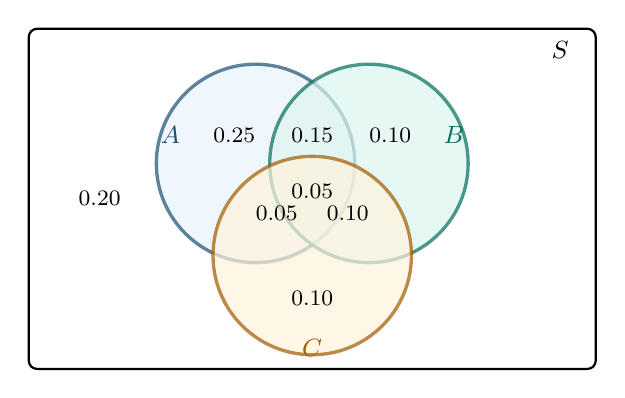
\begin{tikzpicture}[scale=0.9]
  \draw[thick,rounded corners=3pt](-4,-2.4)rectangle(4,2.4);
  \node[font=\small]at(3.5,2.1){$S$};
  \draw[fill=lightbg,draw=primary,line width=1.2pt,opacity=0.7](-0.8,0.5)circle(1.4cm);
  \draw[fill=tealbg,draw=tealclr,line width=1.2pt,opacity=0.7](0.8,0.5)circle(1.4cm);
  \draw[fill=amberbg,draw=amberclr,line width=1.2pt,opacity=0.7](0,-0.8)circle(1.4cm);
  \node[font=\small\bfseries\color{primary}]at(-2.0,0.9){$A$};
  \node[font=\small\bfseries\color{tealclr}]at(2.0,0.9){$B$};
  \node[font=\small\bfseries\color{amberclr}]at(0,-2.1){$C$};
  \node[font=\footnotesize]at(-1.1,0.9){0.25};
  \node[font=\footnotesize]at(1.1,0.9){0.10};
  \node[font=\footnotesize]at(0,-1.4){0.10};
  \node[font=\footnotesize]at(0,0.9){0.15};
  \node[font=\footnotesize]at(-0.5,-0.2){0.05};
  \node[font=\footnotesize]at(0.5,-0.2){0.10};
  \node[font=\footnotesize]at(0,0.1){0.05};
  \node[font=\footnotesize]at(-3.0,0){0.20};
\end{tikzpicture}
\end{center}
$P(A\cup B\cup C)=0.5+0.4+0.3-0.2-0.1-0.15+0.05=0.80$.\; $P(\text{none})=0.20$.
\end{examplebox}

\newpage

%============================================================
%  CHAPTER 3 — CARD GAME PROBABILITY
%============================================================
\begin{tcolorbox}[enhanced,arc=0pt,boxrule=0pt,colback=primary,colframe=primary,
  left=16pt,right=16pt,top=14pt,bottom=10pt,borderline south={4pt}{0pt}{accent}]
  {\color{accent!70}\small\bfseries CHAPTER 03}\\[4pt]
  {\LARGE\bfseries\color{white}Probability --- Card Games}
\end{tcolorbox}
\addcontentsline{toc}{section}{Chapter 3 --- Probability: Card Games}
\vspace{10pt}

\begin{histbox}
Playing cards arrived in Europe from Asia around the 14th century. The standard 52-card deck evolved in France around 1480, where the four suits --- spades ($\spadesuit$), hearts ($\heartsuit$), diamonds ($\diamondsuit$), clubs ($\clubsuit$) --- became standardised. Mathematicians began analysing card games as early as the 17th century; Gerolamo Cardano's \textit{Liber de Ludo Aleae} (c.\ 1560) computed probabilities for dice and cards. The analysis of poker hands was a landmark early application of combinatorial probability. Today, card-based probability problems appear in every undergraduate statistics course as a rich, visual setting to develop probabilistic thinking.
\end{histbox}

\bigskip

\subsection{3.1 Structure of the Standard Deck}

\begin{center}
\begin{tcolorbox}[colback=white,colframe=accent,arc=4pt,boxrule=1.5pt,
  left=8pt,right=8pt,top=8pt,bottom=8pt,
  title={\small\bfseries\color{white}The 52-Card Deck},colbacktitle=primary,
  attach boxed title to top left={xshift=10pt,yshift=-\tcboxedtitleheight/2},
  boxed title style={arc=3pt,boxrule=0pt}]
\begin{center}
{\small\begin{tabular}{|C{2.8cm}|C{2.8cm}|C{2.8cm}|C{2.8cm}|}
\hline\rowcolor{primary}
\hcell{\textcolor{cardred}{$\heartsuit$} Hearts}&\hcell{\textcolor{cardred}{$\diamondsuit$} Diamonds}&\hcell{$\spadesuit$ Spades}&\hcell{$\clubsuit$ Clubs}\\\hline
\textcolor{cardred}{13 cards}&\textcolor{cardred}{13 cards}&13 cards&13 cards\\\hline
\multicolumn{2}{|C{5.8cm}|}{\textbf{Red: 26 cards}}&\multicolumn{2}{C{5.8cm}|}{\textbf{Black: 26 cards}}\\\hline
\end{tabular}}

\bigskip
{\small\begin{tabular}{|l|C{2.5cm}|C{6cm}|}
\hline\rowcolor{primary}\hcell{Category}&\hcell{Count}&\hcell{Cards}\\\hline
Aces & 4 & A\HS\; A\DS\; A\SPS\; A\CS\\\hline
Kings & 4 & K\HS\; K\DS\; K\SPS\; K\CS\\\hline
Queens & 4 & Q\HS\; Q\DS\; Q\SPS\; Q\CS\\\hline
Jacks & 4 & J\HS\; J\DS\; J\SPS\; J\CS\\\hline
Face Cards & 12 & J, Q, K in each of 4 suits\\\hline
Number Cards & 36 & 2--10 in each of 4 suits\\\hline
\end{tabular}}
\end{center}
\medskip\textbf{Sample 5-card hand:}\quad
\mcard{A}{\HS}{cardred}\;\mcard{K}{\SPS}{black}\;\mcard{Q}{\DS}{cardred}\;\mcard{J}{\CS}{black}\;\mcard{10}{\HS}{cardred}
\end{tcolorbox}
\end{center}

\newpage
\subsection{3.2 Single-Card Probabilities}

\begin{examplebox}[Example 3.1 --- Basic Single-Card Draws]
One card drawn at random from a shuffled 52-card deck:

\begin{center}{\small
\begin{tabular}{|l|C{2.2cm}|C{3.2cm}|}
\hline\rowcolor{primary}\hcell{Event}&\hcell{Count}&\hcell{Probability}\\\hline
Ace & 4 & $4/52 = 1/13 \approx 0.077$\\\hline
Heart (\HS) & 13 & $13/52 = 1/4 = 0.25$\\\hline
Face Card (J,Q,K) & 12 & $12/52 = 3/13 \approx 0.231$\\\hline
Red Card & 26 & $26/52 = 1/2 = 0.50$\\\hline
Black Ace & 2 & $2/52 = 1/26 \approx 0.038$\\\hline
Red Face Card & 6 & $6/52 = 3/26 \approx 0.115$\\\hline
Not a King & 48 & $48/52 = 12/13 \approx 0.923$\\\hline
\end{tabular}}
\end{center}
\end{examplebox}

\subsection{3.3 Compound Events and Neither/Nor}

\begin{examplebox}[Example 3.2 --- Union, Intersection, Neither/Nor]
One card drawn. Let $A$ = Queen, $B$ = Spade.\\
$P(A)=4/52$, $P(B)=13/52$, $P(A\cap B)=P(\text{Queen of Spades})=1/52$.\\[6pt]
\textbf{(a) Queen or Spade:}
\[P(A\cup B)=\frac{4+13-1}{52}=\frac{16}{52}=\frac{4}{13}\approx0.308\]
\textbf{(b) Neither Queen nor Spade:}
\[P((A\cup B)^c)=1-\frac{16}{52}=\frac{36}{52}=\frac{9}{13}\approx0.692\]
\textbf{(c) Queen but not Spade:} $P(A\cap B^c)=4/52-1/52=3/52$\\
These are: \mcard{Q}{\HS}{cardred}\;\mcard{Q}{\DS}{cardred}\;\mcard{Q}{\CS}{black}
\end{examplebox}

\begin{examplebox}[Example 3.3 --- Conditional Probability with Cards]
Given the drawn card is a \textbf{Face Card}, find the probability it is a King.\\[6pt]
Face cards (12 total): \mcard{J}{\HS}{cardred}\mcard{Q}{\HS}{cardred}\mcard{K}{\HS}{cardred}\mcard{J}{\DS}{cardred}\mcard{Q}{\DS}{cardred}\mcard{K}{\DS}{cardred}\mcard{J}{\SPS}{black}\mcard{Q}{\SPS}{black}\mcard{K}{\SPS}{black}\mcard{J}{\CS}{black}\mcard{Q}{\CS}{black}\mcard{K}{\CS}{black}\\[6pt]
Kings among face cards: 4.
\[P(\text{King}\mid\text{Face})=\frac{P(\text{King}\cap\text{Face})}{P(\text{Face})}=\frac{4/52}{12/52}=\frac{4}{12}=\frac{1}{3}\approx0.333\]
\end{examplebox}

\subsection{3.4 Drawing Multiple Cards}

\begin{defbox}[With vs Without Replacement]
\textbf{With replacement:} after drawing, the card is returned. Each draw is \textbf{independent}: $P(\text{2nd event})$ unchanged.\\[4pt]
\textbf{Without replacement:} drawn card is \textit{not} returned. Draws are \textbf{dependent}: each draw reduces the deck by one.
\end{defbox}

\begin{examplebox}[Example 3.4 --- Two-Card Draws: With and Without Replacement]
\textbf{Find $P(\text{both Aces})$:}\\[4pt]
\textbf{With replacement:} $P=\dfrac{4}{52}\times\dfrac{4}{52}=\dfrac{16}{2704}=\dfrac{1}{169}\approx0.00592$\\[6pt]
\textbf{Without replacement:} $P=\dfrac{4}{52}\times\dfrac{3}{51}=\dfrac{12}{2652}=\dfrac{1}{221}\approx0.00452$\\[6pt]
The without-replacement probability is lower because one Ace has been removed from the deck.\\[4pt]
\textbf{Find $P(\text{first Ace, second King})$ without replacement:}
\[P=\frac{4}{52}\times\frac{4}{51}=\frac{16}{2652}=\frac{4}{663}\approx0.00603\]
\end{examplebox}

\begin{examplebox}[Example 3.5 --- Three Cards Without Replacement]
Three cards drawn without replacement. Find $P(\text{all three are Hearts})$.
\[P=\frac{13}{52}\times\frac{12}{51}\times\frac{11}{50}=\frac{1716}{132600}=\frac{11}{850}\approx0.01294\]
\end{examplebox}

\subsection{3.5 Five-Card Poker Hands}

\begin{defbox}[Total 5-Card Hands]
$\dbinom{52}{5}=\dfrac{52!}{5!\,47!}=\mathbf{2\,598\,960}$
\end{defbox}

\begin{examplebox}[Example 3.6 --- Poker Hand Probabilities]
\textbf{(a) Royal Flush} (A, K, Q, J, 10 of same suit): 4 ways (one per suit).
\[P=\frac{4}{2\,598\,960}\approx0.00000154\]
\begin{center}\mcard{A}{\HS}{cardred}\mcard{K}{\HS}{cardred}\mcard{Q}{\HS}{cardred}\mcard{J}{\HS}{cardred}\mcard{10}{\HS}{cardred}\end{center}

\textbf{(b) Four of a Kind:} choose rank $\binom{13}{1}$, all 4 suits, plus any 1 of 48 remaining cards.
\[\binom{13}{1}\times1\times48=624 \qquad P\approx0.000240\]
\begin{center}\mcard{K}{\HS}{cardred}\mcard{K}{\DS}{cardred}\mcard{K}{\SPS}{black}\mcard{K}{\CS}{black}\mcard{7}{\DS}{cardred}\end{center}

\textbf{(c) Full House:} choose rank for triple $\binom{13}{1}$, choose 3 suits $\binom{4}{3}$; choose rank for pair $\binom{12}{1}$, choose 2 suits $\binom{4}{2}$.
\[13\times4\times12\times6=3744 \qquad P\approx0.00144\]
\begin{center}\mcard{A}{\HS}{cardred}\mcard{A}{\DS}{cardred}\mcard{A}{\SPS}{black}\mcard{Q}{\CS}{black}\mcard{Q}{\DS}{cardred}\end{center}

\textbf{(d) Flush} (5 same suit, not straight): $4\times\binom{13}{5}-40=5108$. $P\approx0.00197$.\\[4pt]
\textbf{(e) One Pair:} Choose rank $\binom{13}{1}$, suits $\binom{4}{2}$; choose 3 different ranks $\binom{12}{3}$, 1 suit each $4^3$:
\[13\times6\times220\times64=1\,098\,240 \qquad P\approx0.4226\]
\end{examplebox}

\begin{center}{\small
\begin{tabular}{|l|C{2.8cm}|C{2.8cm}|}
\hline\rowcolor{primary}\hcell{Hand}&\hcell{Combinations}&\hcell{Probability}\\\hline
Royal Flush & 4 & 0.00000154\\\hline
Straight Flush & 36 & 0.0000139\\\hline
Four of a Kind & 624 & 0.000240\\\hline
Full House & 3,744 & 0.00144\\\hline
Flush & 5,108 & 0.00197\\\hline
Straight & 10,200 & 0.00392\\\hline
Three of a Kind & 54,912 & 0.0211\\\hline
Two Pair & 123,552 & 0.0475\\\hline
One Pair & 1,098,240 & 0.4226\\\hline
High Card & 1,302,540 & 0.5012\\\hline
\textbf{Total} & \textbf{2,598,960} & \textbf{1.0000}\\\hline
\end{tabular}}
\end{center}

\begin{practicebox}
\begin{enumerate}[label=\textbf{Q\arabic*.},noitemsep]
  \item From 52 cards, find $P(\text{Ace or Club})$.
  \item Three cards drawn without replacement. Find $P(\text{first two red, third black})$.
  \item A card is a red card. Given this, find $P(\text{it is an Ace})$.
  \item Find $P(\text{neither a heart nor a face card})$ when one card is drawn.
  \item Two cards drawn without replacement. Find $P(\text{exactly one Ace})$.
\end{enumerate}
\end{practicebox}

\newpage

%============================================================
%  CHAPTER 4 — DESCRIPTIVE STATISTICS
%============================================================
\begin{tcolorbox}[enhanced,arc=0pt,boxrule=0pt,colback=primary,colframe=primary,
  left=16pt,right=16pt,top=14pt,bottom=10pt,borderline south={4pt}{0pt}{accent}]
  {\color{accent!70}\small\bfseries CHAPTER 04}\\[4pt]
  {\LARGE\bfseries\color{white}Descriptive Statistics}
\end{tcolorbox}
\addcontentsline{toc}{section}{Chapter 4 --- Descriptive Statistics}
\vspace{10pt}

\subsection{4.1 Frequency Distributions}

\begin{defbox}[Frequency Distribution]
A \textbf{frequency distribution} organises raw data into classes. For each class $[L_i, U_i)$:
\begin{itemize}[noitemsep]
  \item \textbf{Midpoint:} $m_i=(L_i+U_i)/2$
  \item \textbf{Frequency} $f_i$: number of observations in class $i$
  \item \textbf{Cumulative Frequency} $F_i=\sum_{j\leq i}f_j$
  \item \textbf{Relative Frequency:} $f_i/n$
\end{itemize}
\end{defbox}

\subsection{4.2 Measures of Central Tendency}

\begin{defbox}[Arithmetic Mean]
\textbf{Ungrouped:} $\bar x=\dfrac{\sum_{i=1}^n x_i}{n}$\\[8pt]
\textbf{Grouped:} $\bar x=\dfrac{\sum f_i m_i}{\sum f_i}$ where $m_i$ is the class midpoint.\\[4pt]
Properties: (i) $\sum(x_i-\bar x)=0$;\quad (ii) $\sum(x_i-\bar x)^2$ is minimised by $\bar x$;\quad (iii) affected by outliers.
\end{defbox}

\begin{defbox}[Median]
The \textbf{median} is the middle value of ordered data. For grouped data:
\[
\text{Median} = L + \frac{h}{f}\!\left(\frac{N}{2}-F\right)
\]
where $L$ = lower boundary of median class, $h$ = class width, $f$ = frequency of median class, $F$ = cumulative frequency before median class, $N=\sum f$.\\[4pt]
\textbf{Median class:} the class containing the $N/2$-th observation.
\end{defbox}

\begin{defbox}[Mode]
The \textbf{mode} is the most frequently occurring value. For grouped data:
\[
\text{Mode} = L + h\cdot\frac{f_1-f_0}{(f_1-f_0)+(f_1-f_2)}
\]
where $f_1$ = modal class frequency, $f_0$ = frequency before, $f_2$ = frequency after.
\end{defbox}

\subsection{4.3 Measures of Dispersion}

\begin{defbox}[Mean Deviation]
\[\text{MD from mean}=\frac{\sum f_i|m_i-\bar x|}{\sum f_i}\]
\textbf{Coefficient of Mean Deviation:} $\;\text{Cmd}=\dfrac{\text{MD}}{\bar x}$
\end{defbox}

\begin{defbox}[Variance and Standard Deviation]
\textbf{Ungrouped (sample):}
\[s^2=\frac{\sum(x_i-\bar x)^2}{n-1}=\frac{\sum x_i^2-n\bar x^2}{n-1}\]
\textbf{Grouped (sample):}
\[s^2=\frac{\sum f_i(m_i-\bar x)^2}{\sum f_i-1}\]
Standard deviation $s=\sqrt{s^2}$. The division by $n-1$ (not $n$) makes $s^2$ an \textit{unbiased} estimator of $\sigma^2$.
\end{defbox}

\begin{defbox}[Coefficient of Variation and Coefficient of Standard Deviation]
\[\text{CV}=\frac{s}{\bar x}\times100\%\qquad\text{Coefficient of SD}=\frac{s}{\bar x}\]
These are \textbf{dimensionless} measures that allow comparison of variability across datasets with different units or different means.\\[4pt]
\textbf{Lower CV $\Rightarrow$ more homogeneous, more consistent dataset.}
\end{defbox}

\begin{examplebox}[Example 4.1 --- Full Descriptive Analysis from Grouped Data]
Marks of 50 students in a statistics test:
\begin{center}{\small
\begin{tabular}{|C{2cm}|C{1.2cm}|C{1.5cm}|C{1.5cm}|C{2cm}|C{2.5cm}|}
\hline\rowcolor{primary}
\hcell{Class}&\hcell{$f_i$}&\hcell{$m_i$}&\hcell{$F_i$}&\hcell{$f_im_i$}&\hcell{$f_i(m_i-\bar x)^2$}\\\hline
10--20&3&15&3&45&---\\\hline
20--30&7&25&10&175&---\\\hline
30--40&15&35&25&525&---\\\hline
40--50&12&45&37&540&---\\\hline
50--60&8&55&45&440&---\\\hline
60--70&5&65&50&325&---\\\hline
\rowcolor{lightbg}\textbf{Total}&\textbf{50}&&\textbf{}&\textbf{2050}&\\\hline
\end{tabular}}
\end{center}
\textbf{Mean:} $\bar x=2050/50=41.0$

\medskip
\textbf{Median} ($N/2=25$): 25th obs falls in 30--40 ($F=10$, $f=15$).
\[\text{Median}=30+\frac{10}{15}(25-10)=30+10=\mathbf{40.0}\]

\textbf{$Q_1$} ($N/4=12.5$): class 30--40 ($F=10$, $f=15$).
\[Q_1=30+\frac{10}{15}(12.5-10)=30+1.67=\mathbf{31.67}\]

\textbf{$Q_3$} ($3N/4=37.5$): class 40--50 ($F=25$, $f=12$).
\[Q_3=40+\frac{10}{12}(37.5-25)=40+10.42=\mathbf{50.42}\]

Now computing $f_i(m_i-41)^2$: $3(676)+7(256)+15(36)+12(16)+8(196)+5(576)=2028+1792+540+192+1568+2880=\mathbf{8200}$\\[4pt]
$s^2=8200/49=167.35$;\quad $s=\sqrt{167.35}=\mathbf{12.94}$;\quad CV$=12.94/41\times100=\mathbf{31.6\%}$
\end{examplebox}

\subsection{4.4 Measures of Position}

\begin{defbox}[General Interpolation Formula]
For quartiles ($k=4$), deciles ($k=10$), percentiles ($k=100$):
\[
M_r = L + \frac{h}{f}\!\left(\frac{rN}{k}-F\right)
\]
\begin{itemize}[noitemsep]
  \item $r$ = required number (e.g.\ $r=1$ for $Q_1$, $r=3$ for $D_3$, $r=75$ for $P_{75}$)
  \item $L$ = lower class boundary of required class
  \item $h$ = class width; $f$ = class frequency; $F$ = cumulative frequency before required class
\end{itemize}
\end{defbox}

\begin{examplebox}[Example 4.2 --- Deciles and Percentiles]
Using the data from Example 4.1 ($N=50$):

\textbf{$D_3$} ($3N/10=15$): class 30--40 ($F=10$, $f=15$).
\[D_3=30+\frac{10}{15}(15-10)=30+3.33=\mathbf{33.33}\]

\textbf{$D_7$} ($7N/10=35$): class 40--50 ($F=25$, $f=12$).
\[D_7=40+\frac{10}{12}(35-25)=40+8.33=\mathbf{48.33}\]

\textbf{$P_{60}$} ($60N/100=30$): class 40--50 ($F=25$, $f=12$).
\[P_{60}=40+\frac{10}{12}(30-25)=40+4.17=\mathbf{44.17}\]

\textbf{$P_{85}$} ($85N/100=42.5$): class 50--60 ($F=37$, $f=8$).
\[P_{85}=50+\frac{10}{8}(42.5-37)=50+6.875=\mathbf{56.88}\]
\end{examplebox}

\begin{examplebox}[Example 4.3 --- Comparing Consistency of Two Groups]
Test scores of two sections (30 students each):

\begin{center}{\small
\begin{tabular}{|l|C{1.5cm}|C{1.5cm}|C{1.5cm}|C{1.5cm}|C{1.5cm}|}
\hline\rowcolor{primary}
\hcell{Section}&\hcell{$\bar x$}&\hcell{$s$}&\hcell{CV}&\hcell{MD}&\hcell{Cmd}\\\hline
A (Morning)&65.4&8.2&12.5\%&6.8&0.104\\\hline
B (Evening)&72.1&14.6&20.2\%&11.9&0.165\\\hline
\end{tabular}}
\end{center}
\textbf{Conclusion:} Section B has a higher mean but Section A is more consistent --- lower CV and Cmd indicate less variability relative to the mean. Section A students are more homogeneous in performance.
\end{examplebox}

\begin{practicebox}
\begin{enumerate}[label=\textbf{Q\arabic*.},noitemsep]
  \item Given $\bar x=45$, $s=9$, find the CV and interpret it.
  \item For grouped data with $N=80$: find the median class if cumulative frequencies are 12, 28, 55, 70, 80.
  \item Two machines: Machine A ($\bar x=200$ units, $s=15$); Machine B ($\bar x=185$ units, $s=10$). Which is more consistent?
  \item Compute $Q_2$, $D_5$, and $P_{50}$ for any dataset and comment on the relationship.
\end{enumerate}
\end{practicebox}

\newpage

%============================================================
%  CHAPTER 5 — SAMPLING DISTRIBUTIONS
%============================================================
\begin{tcolorbox}[enhanced,arc=0pt,boxrule=0pt,colback=primary,colframe=primary,
  left=16pt,right=16pt,top=14pt,bottom=10pt,borderline south={4pt}{0pt}{accent}]
  {\color{accent!70}\small\bfseries CHAPTER 05}\\[4pt]
  {\LARGE\bfseries\color{white}Sampling Distributions}
\end{tcolorbox}
\addcontentsline{toc}{section}{Chapter 5 --- Sampling Distributions}
\vspace{10pt}

\begin{histbox}
The concept of a sampling distribution was implicit in the work of \textbf{Abraham de Moivre} (1733), who proved the normal approximation to the binomial. \textbf{Carl Friedrich Gauss} (1809) derived the normal distribution in the context of measurement errors. The $\chi^2$ distribution was characterised by \textbf{Karl Pearson} in 1900. \textbf{William S.\ Gosset} (writing as ``Student'', 1908) derived the $t$-distribution while working at Guinness Brewery --- he needed to handle small samples in quality control. \textbf{R.\ A.\ Fisher} introduced the $F$-distribution (1924) and proved the independence of $\bar X$ and $s^2$ for normal populations. The Central Limit Theorem in its modern form is due to \textbf{Aleksandr Lyapunov} (1901) and \textbf{Jarl Waldemar Lindeberg} (1922).
\end{histbox}

\bigskip

\begin{defbox}[Sampling Distribution]
The \textbf{sampling distribution} of a statistic $T=T(X_1,\ldots,X_n)$ is its probability distribution over all possible samples of size $n$ from the population.\\[6pt]
For the sample mean $\bar X$:
\[E(\bar X)=\mu, \qquad \text{Var}(\bar X)=\frac{\sigma^2}{n}, \qquad \text{SE}(\bar X)=\frac{\sigma}{\sqrt{n}}\]
The standard error \textbf{decreases} as $n$ increases --- larger samples give more precise estimates.
\end{defbox}

\subsection{5.1 Normal Distribution}

\begin{defbox}[Normal Distribution $N(\mu,\sigma^2)$]
\[f(x)=\frac{1}{\sigma\sqrt{2\pi}}\exp\!\left(-\frac{(x-\mu)^2}{2\sigma^2}\right), \quad -\infty<x<\infty\]
\textbf{Standard Normal:} $Z=\dfrac{X-\mu}{\sigma}\sim N(0,1)$. CDF: $\Phi(z)=P(Z\leq z)$.\\[6pt]
\textbf{Properties:} symmetric about $\mu$; mean = median = mode = $\mu$; total area = 1; bell-shaped.\\[4pt]
\textbf{Empirical Rule (68-95-99.7):}\\
$P(\mu-\sigma<X<\mu+\sigma)\approx68\%$;\quad $P(\mu-2\sigma<X<\mu+2\sigma)\approx95\%$;\quad $P(\mu-3\sigma<X<\mu+3\sigma)\approx99.7\%$
\end{defbox}

\begin{examplebox}[Example 5.1 --- Normal Probability Calculations]
$X\sim N(60,100)$ (mean 60, $\sigma=10$). Find:

\textbf{(a)} $P(X<75)=P\!\left(Z<\frac{75-60}{10}\right)=P(Z<1.5)=\Phi(1.5)=0.9332$

\textbf{(b)} $P(50<X<70)=P(-1<Z<1)=\Phi(1)-\Phi(-1)=0.8413-0.1587=\mathbf{0.6827}$

\textbf{(c)} $P(X>80)=P(Z>2)=1-0.9772=\mathbf{0.0228}$

\textbf{(d)} Find $x$ such that $P(X<x)=0.90$: $Z_{0.90}=1.282$, so $x=60+1.282(10)=\mathbf{72.82}$
\end{examplebox}

\subsection{5.2 Chi-Square Distribution}

\begin{defbox}[$\chi^2$ Distribution]
If $Z_1,\ldots,Z_k\overset{iid}{\sim}N(0,1)$ then:
\[\chi^2=\sum_{i=1}^k Z_i^2\sim\chi^2(k)\]
PDF: $f(x)=\dfrac{x^{k/2-1}e^{-x/2}}{2^{k/2}\Gamma(k/2)}$, $x>0$.\\[6pt]
Mean $=k$, Variance $=2k$. \textbf{Right-skewed}; approaches normality as $k\to\infty$.\\[6pt]
\textbf{Key result:} If $X_1,\ldots,X_n\overset{iid}{\sim}N(\mu,\sigma^2)$, then:
\[\frac{(n-1)s^2}{\sigma^2}\sim\chi^2(n-1)\]
and $\bar X$ and $s^2$ are \textbf{independent} (Fisher's theorem, 1925).
\end{defbox}

\begin{derivbox}[Why $(n-1)$ Degrees of Freedom?]
$\sum(X_i-\bar X)^2$ involves $n$ terms subject to the constraint $\sum(X_i-\bar X)=0$, leaving $n-1$ free terms. Each standardised free term contributes one chi-square degree of freedom. The constraint ``costs'' one degree of freedom.
\end{derivbox}

\subsection{5.3 Student's $t$-Distribution}

\begin{defbox}[$t$-Distribution $t(\nu)$]
If $Z\sim N(0,1)$ and $V\sim\chi^2(\nu)$ are \textbf{independent}:
\[T=\frac{Z}{\sqrt{V/\nu}}\sim t(\nu)\]
PDF: $f(t)=\dfrac{\Gamma\!\left(\frac{\nu+1}{2}\right)}{\sqrt{\nu\pi}\,\Gamma\!\left(\frac{\nu}{2}\right)}\!\left(1+\frac{t^2}{\nu}\right)^{-(\nu+1)/2}$\\[6pt]
Properties: symmetric about 0; heavier tails than $N(0,1)$; as $\nu\to\infty$, $t(\nu)\to N(0,1)$.\\[6pt]
\textbf{Practical form:} When $\sigma$ is unknown and $X_i\sim N(\mu,\sigma^2)$:
\[T=\frac{\bar X-\mu}{s/\sqrt{n}}\sim t(n-1)\]
\end{defbox}

\begin{derivbox}[Derivation of the $t$-Statistic]
Since $\bar X\sim N(\mu,\sigma^2/n)$: $Z=\dfrac{\bar X-\mu}{\sigma/\sqrt{n}}\sim N(0,1)$.\\
And $V=\dfrac{(n-1)s^2}{\sigma^2}\sim\chi^2(n-1)$, independent of $Z$.\\
Therefore: $T=\dfrac{Z}{\sqrt{V/(n-1)}}=\dfrac{(\bar X-\mu)/(\sigma/\sqrt{n})}{\sqrt{(n-1)s^2/\sigma^2/(n-1)}}=\dfrac{\bar X-\mu}{s/\sqrt{n}}\sim t(n-1)$. \hfill$\square$
\end{derivbox}

\subsection{5.4 $F$-Distribution}

\begin{defbox}[$F$-Distribution $F(m,n)$]
If $U\sim\chi^2(m)$ and $V\sim\chi^2(n)$ are independent:
\[F=\frac{U/m}{V/n}\sim F(m,n)\]
Mean $=n/(n-2)$ for $n>2$. Right-skewed. \textbf{Key property:} $1/F\sim F(n,m)$.\\[4pt]
\textbf{Use:} $F=s_1^2/s_2^2\sim F(n_1-1,n_2-1)$ to compare two population variances.
\end{defbox}

\subsection{5.5 Central Limit Theorem}

\begin{thmbox}[Central Limit Theorem (CLT)]
Let $X_1,X_2,\ldots,X_n$ be iid with mean $\mu$ and finite variance $\sigma^2$. Then:
\[\frac{\bar X-\mu}{\sigma/\sqrt{n}}\xrightarrow{d}N(0,1)\quad\text{as }n\to\infty\]
equivalently $\bar X\overset{\text{approx}}{\sim}N(\mu,\sigma^2/n)$ for large $n$.\\[6pt]
\textbf{Proof sketch (Lindeberg-Lévy):} The moment generating function (MGF) of $\bar X$ standardised converges pointwise to $e^{t^2/2}$, the MGF of $N(0,1)$. Convergence of MGFs implies convergence in distribution. \hfill$\square$\\[4pt]
\textbf{Rule of thumb:} $n\geq30$ usually sufficient. For proportions, need $np\geq5$ and $n(1-p)\geq5$.
\end{thmbox}

\begin{examplebox}[Example 5.2 --- CLT in Practice]
Incomes in a city: $\mu=\$45000$, $\sigma=\$12000$. A sample of $n=100$ is taken.\\[4pt]
By CLT: $\bar X\sim N(45000,\,12000^2/100)=N(45000,\,1200^2)$.\\[6pt]
\textbf{(a)} $P(\bar X>47000)=P\!\left(Z>\frac{47000-45000}{1200}\right)=P(Z>1.67)=1-0.9525=\mathbf{0.0475}$\\[6pt]
\textbf{(b)} $P(44000<\bar X<46000)=P\!\left(\frac{-1000}{1200}<Z<\frac{1000}{1200}\right)=P(-0.83<Z<0.83)$\\
$=2\Phi(0.83)-1=2(0.7967)-1=\mathbf{0.5934}$
\end{examplebox}

\begin{center}{\small
\begin{tabular}{|l|C{2cm}|C{2cm}|C{2.5cm}|C{2.5cm}|}
\hline\rowcolor{primary}\hcell{Distribution}&\hcell{Symbol}&\hcell{Parameters}&\hcell{Mean}&\hcell{Variance}\\\hline
Normal&$N(\mu,\sigma^2)$&$\mu,\sigma^2$&$\mu$&$\sigma^2$\\\hline
Chi-Square&$\chi^2(k)$&$k$ (df)&$k$&$2k$\\\hline
Student's $t$&$t(\nu)$&$\nu$ (df)&0 ($\nu>1$)&$\nu/(\nu-2)$ ($\nu>2$)\\\hline
F&$F(m,n)$&$m,n$ (df)&$n/(n-2)$&---\\\hline
\end{tabular}}
\end{center}

\newpage

%============================================================
%  CHAPTER 6 — POINT ESTIMATION
%============================================================
\begin{tcolorbox}[enhanced,arc=0pt,boxrule=0pt,colback=primary,colframe=primary,
  left=16pt,right=16pt,top=14pt,bottom=10pt,borderline south={4pt}{0pt}{accent}]
  {\color{accent!70}\small\bfseries CHAPTER 06}\\[4pt]
  {\LARGE\bfseries\color{white}Point Estimation}
\end{tcolorbox}
\addcontentsline{toc}{section}{Chapter 6 --- Point Estimation}
\vspace{10pt}

\begin{histbox}
The theory of estimation was systematised by \textbf{R.\ A.\ Fisher}, who introduced \textit{maximum likelihood estimation} (1912, 1922), \textit{sufficiency} (1920), and the \textit{information inequality} (1925). \textbf{C.\ R.\ Rao} and \textbf{Harald Cramér} independently derived the lower bound for the variance of unbiased estimators (1945--1946). \textbf{David Blackwell} proved his conditioning theorem (1947), and \textbf{Erich Lehmann} with \textbf{Henry Scheffé} combined it with completeness to characterise the unique minimum-variance unbiased estimator (1950).
\end{histbox}

\bigskip

\begin{defbox}[Point Estimator and Estimate]
A \textbf{point estimator} $\hat\theta=T(X_1,\ldots,X_n)$ is a statistic used to estimate the unknown parameter $\theta$. A specific computed value $\hat\theta=T(x_1,\ldots,x_n)$ is a \textbf{point estimate}.
\end{defbox}

\subsection{6.1 Properties of Estimators}

\begin{defbox}[Unbiasedness]
$\hat\theta$ is \textbf{unbiased} for $\theta$ if $E(\hat\theta)=\theta$ for all $\theta$.\\[4pt]
$\text{Bias}(\hat\theta)=E(\hat\theta)-\theta$. An unbiased estimator has zero bias.\\[6pt]
\textbf{Examples:}\\
$\bar X$ is unbiased for $\mu$: $E(\bar X)=\mu$. \checkmark\\
$s^2=\sum(X_i-\bar X)^2/(n-1)$ is unbiased for $\sigma^2$: $E(s^2)=\sigma^2$. \checkmark\\
$\hat\sigma^2_{MLE}=\sum(X_i-\bar X)^2/n$ is \textit{biased}: $E(\hat\sigma^2_{MLE})=\dfrac{n-1}{n}\sigma^2\neq\sigma^2$. $\times$
\end{defbox}

\begin{defbox}[Mean Squared Error (MSE)]
\[\text{MSE}(\hat\theta)=E\!\left[(\hat\theta-\theta)^2\right]=\text{Var}(\hat\theta)+[\text{Bias}(\hat\theta)]^2\]
For unbiased estimators: MSE $=$ Variance. The MSE captures both bias and variance simultaneously.\\[4pt]
A \textbf{biased} estimator can have smaller MSE than an unbiased one if its variance is sufficiently small.
\end{defbox}

\begin{defbox}[Consistency]
$\hat\theta_n$ is \textbf{consistent} for $\theta$ if $\hat\theta_n\xrightarrow{P}\theta$, i.e.\ $\forall\varepsilon>0$: $\lim_{n\to\infty}P(|\hat\theta_n-\theta|>\varepsilon)=0$.\\[4pt]
\textbf{Sufficient condition:} $\text{MSE}(\hat\theta_n)\to0$ as $n\to\infty$.\\[4pt]
$\bar X$ is consistent: $\text{MSE}(\bar X)=\sigma^2/n\to0$.
\end{defbox}

\begin{defbox}[Relative Efficiency]
Among unbiased estimators $\hat\theta_1$ and $\hat\theta_2$, the \textbf{relative efficiency} of $\hat\theta_1$ relative to $\hat\theta_2$ is:
\[\text{eff}(\hat\theta_1,\hat\theta_2)=\frac{\text{Var}(\hat\theta_2)}{\text{Var}(\hat\theta_1)}\]
$\hat\theta_1$ is \textbf{more efficient} if eff $>1$. The most efficient estimator is called the \textbf{UMVUE} (Uniformly Minimum Variance Unbiased Estimator).
\end{defbox}

\begin{defbox}[Sufficiency and Factorization Theorem]
A statistic $T(\mathbf X)$ is \textbf{sufficient} for $\theta$ if the conditional distribution of $\mathbf X$ given $T=t$ does not depend on $\theta$ --- $T$ contains \textit{all the information} about $\theta$ in the sample.\\[6pt]
\textbf{Neyman Factorization Theorem:} $T$ is sufficient for $\theta$ iff the joint pdf/pmf factors as:
\[f(\mathbf x;\theta)=g(T(\mathbf x),\theta)\cdot h(\mathbf x)\]
where $g$ depends on the data \textit{only through} $T$, and $h$ does not depend on $\theta$.
\end{defbox}

\begin{examplebox}[Example 6.1 --- Sufficiency via Factorization]
\textbf{Bernoulli:} $X_i\sim\text{Bernoulli}(p)$. Joint pmf:
\[f(\mathbf x;p)=p^{\sum x_i}(1-p)^{n-\sum x_i}=\underbrace{p^T(1-p)^{n-T}}_{g(T,p)}\cdot\underbrace{1}_{h(\mathbf x)}\]
where $T=\sum X_i$. By factorization, $T=\sum X_i$ is \textbf{sufficient} for $p$.\\[6pt]
\textbf{Normal:} For $X_i\sim N(\mu,\sigma^2)$ with $\sigma^2$ known, $\bar X$ is sufficient for $\mu$.\\
For both $\mu$ and $\sigma^2$ unknown, $(\bar X, s^2)$ jointly form a \textbf{complete sufficient} statistic.
\end{examplebox}

\subsection{6.2 Cramer-Rao Lower Bound}

\begin{thmbox}[Cramer-Rao Lower Bound (CRLB)]
Under regularity conditions, for any unbiased estimator $\hat\theta$ of $\theta$:
\[\text{Var}(\hat\theta)\geq\frac{1}{nI(\theta)}\]
where the \textbf{Fisher Information} is:
\[I(\theta)=E\!\left[\left(\frac{\partial\ln f(X;\theta)}{\partial\theta}\right)^2\right]=-E\!\left[\frac{\partial^2\ln f(X;\theta)}{\partial\theta^2}\right]\]
An unbiased estimator achieving the CRLB is called \textbf{efficient} (and is automatically the UMVUE).
\end{thmbox}

\begin{derivbox}[Proof of CRLB]
Under regularity (interchange differentiation and integration):
$E\!\left[\frac{\partial\ln f}{\partial\theta}\right]=0$ (score has mean zero).\\
By Cauchy-Schwarz: $\left[\text{Cov}\!\left(\hat\theta,\,\frac{\partial\ln f}{\partial\theta}\right)\right]^2\leq\text{Var}(\hat\theta)\cdot\text{Var}\!\left(\frac{\partial\ln f}{\partial\theta}\right)$\\[4pt]
The left side equals $[\partial E(\hat\theta)/\partial\theta]^2=[1]^2=1$ (since $\hat\theta$ is unbiased).\\
The right side gives $\text{Var}(\hat\theta)\cdot nI(\theta)\geq1$, so $\text{Var}(\hat\theta)\geq1/(nI(\theta))$. \hfill$\square$
\end{derivbox}

\begin{examplebox}[Example 6.2 --- CRLB for Normal Mean]
$X\sim N(\mu,\sigma^2)$, $\sigma^2$ known. $\ln f=-\frac{1}{2}\ln(2\pi\sigma^2)-\frac{(x-\mu)^2}{2\sigma^2}$.\\[4pt]
$\dfrac{\partial^2\ln f}{\partial\mu^2}=-\dfrac{1}{\sigma^2}$, so $I(\mu)=1/\sigma^2$.\\[4pt]
CRLB $=\sigma^2/n$. Since $\text{Var}(\bar X)=\sigma^2/n$, $\bar X$ \textbf{is efficient} for $\mu$.
\end{examplebox}

\begin{examplebox}[Example 6.3 --- CRLB for Poisson]
$X\sim\text{Poisson}(\lambda)$. $\ln f=x\ln\lambda-\lambda-\ln(x!)$.\\[4pt]
$\dfrac{\partial^2\ln f}{\partial\lambda^2}=-x/\lambda^2$, so $I(\lambda)=E(X)/\lambda^2=1/\lambda$.\\[4pt]
CRLB $=\lambda/n$. Since $\text{Var}(\bar X)=\lambda/n$, $\bar X$ \textbf{is efficient} for $\lambda$.
\end{examplebox}

\subsection{6.3 Rao-Blackwell and Lehmann-Scheff\'e Theorems}

\begin{thmbox}[Rao-Blackwell Theorem (1947)]
Let $\hat\theta$ be any unbiased estimator of $\theta$ and $T$ a sufficient statistic. Define:
\[\hat\theta^*=E(\hat\theta\mid T)\]
Then $\hat\theta^*$ is: (i) a statistic (function of data only); (ii) unbiased: $E(\hat\theta^*)=\theta$; (iii) at least as efficient: $\text{Var}(\hat\theta^*)\leq\text{Var}(\hat\theta)$.\\[4pt]
\textbf{Proof of (iii):} By Eve's law: $\text{Var}(\hat\theta)=E[\text{Var}(\hat\theta\mid T)]+\text{Var}[E(\hat\theta\mid T)]=E[\text{Var}(\hat\theta\mid T)]+\text{Var}(\hat\theta^*)\geq\text{Var}(\hat\theta^*)$. \hfill$\square$
\end{thmbox}

\begin{thmbox}[Lehmann-Scheff\'e Theorem (1950)]
If $T$ is a \textbf{complete sufficient} statistic and $\hat\theta^*=E(\hat\theta\mid T)$ is unbiased for $\theta$, then $\hat\theta^*$ is the \textbf{unique UMVUE} of $\theta$.
\end{thmbox}

\subsection{6.4 Method of Moments (MOM)}

\begin{defbox}[Method of Moments]
\textbf{Population $r$-th moment:} $\mu_r'=E(X^r)$\\
\textbf{Sample $r$-th moment:} $m_r'=\dfrac{1}{n}\sum_{i=1}^n X_i^r$\\[6pt]
\textbf{MOM:} Set $\mu_r'=m_r'$ for $r=1,2,\ldots,k$ (where $k$ = number of parameters) and solve for the parameters.
\end{defbox}

\begin{examplebox}[Example 6.4 --- MOM Estimators]
\textbf{(a) Normal} $N(\mu,\sigma^2)$: Two parameters, use two moments.\\
$\mu_1'=\mu\;\Rightarrow\;\hat\mu=\bar X$. \quad $\mu_2'=\sigma^2+\mu^2\;\Rightarrow\;\hat\sigma^2=m_2'-\bar X^2=\frac{1}{n}\sum X_i^2-\bar X^2=\frac{1}{n}\sum(X_i-\bar X)^2$

\medskip
\textbf{(b) Exponential} Exp$(\lambda)$: $E(X)=1/\lambda\;\Rightarrow\;\hat\lambda_{MOM}=1/\bar X$.

\medskip
\textbf{(c) Gamma} $(\alpha,\beta)$: $E(X)=\alpha\beta$ and $\text{Var}(X)=\alpha\beta^2$.\\
$\hat\beta=s^2/\bar X$, \quad $\hat\alpha=\bar X^2/s^2$.
\end{examplebox}

\begin{prosbox}
\begin{itemize}[noitemsep]
  \item Simple to compute --- always produces an estimator
  \item No distributional assumptions beyond moment existence
  \item Consistent estimators under mild conditions
\end{itemize}
\end{prosbox}

\begin{consbox}
\begin{itemize}[noitemsep]
  \item Not always efficient (can have larger variance than MLE)
  \item Estimates may fall outside the parameter space (e.g.\ negative variance estimate)
  \item Ignores the full likelihood information
\end{itemize}
\end{consbox}

\subsection{6.5 Maximum Likelihood Estimation (MLE)}

\begin{defbox}[Likelihood and MLE]
Given observations $x_1,\ldots,x_n$, the \textbf{likelihood function} is:
\[L(\theta)=L(\theta;\mathbf x)=\prod_{i=1}^n f(x_i;\theta)\]
The \textbf{log-likelihood} is $\ell(\theta)=\ln L(\theta)=\sum_{i=1}^n\ln f(x_i;\theta)$.\\[6pt]
The \textbf{MLE} $\hat\theta$ maximises $L(\theta)$ (equivalently $\ell(\theta)$). \textbf{Score equation:} $\dfrac{\partial\ell}{\partial\theta}=0$.
\end{defbox}

\begin{keybox}
\textbf{Properties of MLE:}
\begin{itemize}[noitemsep]
  \item \textbf{Consistent:} $\hat\theta_{MLE}\xrightarrow{P}\theta$ as $n\to\infty$
  \item \textbf{Asymptotically Normal:} $\sqrt{n}(\hat\theta-\theta)\xrightarrow{d}N(0,1/I(\theta))$
  \item \textbf{Asymptotically Efficient:} achieves CRLB as $n\to\infty$
  \item \textbf{Invariance:} if $\hat\theta$ is MLE of $\theta$, then $g(\hat\theta)$ is MLE of $g(\theta)$
\end{itemize}
\end{keybox}

\begin{examplebox}[Example 6.5 --- MLE for Binomial, Exponential, Normal]
\textbf{(a) Binomial:} $X\sim B(n,p)$. $\ell(p)=x\ln p+(n-x)\ln(1-p)$.\\
$d\ell/dp=x/p-(n-x)/(1-p)=0\;\Rightarrow\;\boxed{\hat p=x/n}$\\[6pt]
\textbf{(b) Exponential:} $f(x;\lambda)=\lambda e^{-\lambda x}$. $\ell(\lambda)=n\ln\lambda-\lambda\sum x_i$.\\
$d\ell/d\lambda=n/\lambda-\sum x_i=0\;\Rightarrow\;\boxed{\hat\lambda=1/\bar x}$\\[6pt]
\textbf{(c) Normal} ($\mu,\sigma^2$ both unknown):
$\ell=-\frac{n}{2}\ln(2\pi\sigma^2)-\frac{1}{2\sigma^2}\sum(x_i-\mu)^2$\\
$\partial\ell/\partial\mu=0\;\Rightarrow\;\hat\mu=\bar x$;\quad $\partial\ell/\partial\sigma^2=0\;\Rightarrow\;\hat\sigma^2=\frac{1}{n}\sum(x_i-\bar x)^2$ (biased)\\[6pt]
\textbf{(d) Uniform} $U(0,\theta)$: $L(\theta)=\theta^{-n}$ for $\theta\geq x_{(n)}$. $L$ is decreasing in $\theta$, so minimize over valid values: $\boxed{\hat\theta=X_{(n)}=\max(X_i)}$.\\
Note: $E(X_{(n)})=\frac{n}{n+1}\theta$ --- biased. Unbiased version: $\frac{n+1}{n}X_{(n)}$.
\end{examplebox}

\begin{practicebox}
\begin{enumerate}[label=\textbf{Q\arabic*.},noitemsep]
  \item Find MLE of $p$ for the Geometric distribution $P(X=x)=p(1-p)^{x-1}$.
  \item Show $\bar X$ is unbiased and efficient for $\mu$ when $X_i\sim N(\mu,\sigma^2)$ with $\sigma^2$ known.
  \item Compute CRLB for estimating $\lambda$ in the Exponential distribution.
  \item Find MOM and MLE estimators for $\theta$ in $f(x;\theta)=(\theta+1)x^\theta$, $0<x<1$.
\end{enumerate}
\end{practicebox}

\newpage

%============================================================
%  CHAPTER 7 — INTERVAL ESTIMATION
%============================================================
\begin{tcolorbox}[enhanced,arc=0pt,boxrule=0pt,colback=primary,colframe=primary,
  left=16pt,right=16pt,top=14pt,bottom=10pt,borderline south={4pt}{0pt}{accent}]
  {\color{accent!70}\small\bfseries CHAPTER 07}\\[4pt]
  {\LARGE\bfseries\color{white}Interval Estimation}
\end{tcolorbox}
\addcontentsline{toc}{section}{Chapter 7 --- Interval Estimation}
\vspace{10pt}

\begin{defbox}[Confidence Interval]
A \textbf{$(1-\alpha)\times100\%$ confidence interval (CI)} for $\theta$ is a random interval $(L,U)$ where $L$ and $U$ are statistics satisfying:
\[P(L\leq\theta\leq U)=1-\alpha\]
\textbf{Interpretation:} If we constructed such intervals from infinitely many samples, $(1-\alpha)\times100\%$ of them would contain the true parameter. It is \textit{incorrect} to say ``there is $(1-\alpha)$ probability that $\theta$ lies in $(L,U)$'' for a specific realised interval --- $\theta$ is fixed (frequentist view).\\[4pt]
$(1-\alpha)$ = \textbf{confidence level}; \quad $\alpha$ = \textbf{significance level};\quad $E=z_{\alpha/2}\cdot\text{SE}$ = \textbf{margin of error}.
\end{defbox}

\begin{defbox}[Pivotal Quantity Method]
A \textbf{pivot} $Q(\mathbf X,\theta)$ is a function of the data and $\theta$ whose distribution does not depend on $\theta$.\\[4pt]
\textbf{Method:} Find $Q$; find $c_1,c_2$ with $P(c_1\leq Q\leq c_2)=1-\alpha$; rearrange to isolate $\theta$.
\end{defbox}

\subsection{7.1 CI for Mean}

\begin{derivbox}[Derivation of CI for $\mu$ ($\sigma$ known)]
Pivot: $Z=\dfrac{\bar X-\mu}{\sigma/\sqrt n}\sim N(0,1)$.\\[4pt]
$P\!\left(-z_{\alpha/2}\leq\dfrac{\bar X-\mu}{\sigma/\sqrt n}\leq z_{\alpha/2}\right)=1-\alpha$\\[4pt]
Rearranging: $P\!\left(\bar X-z_{\alpha/2}\dfrac{\sigma}{\sqrt n}\leq\mu\leq\bar X+z_{\alpha/2}\dfrac{\sigma}{\sqrt n}\right)=1-\alpha$
\end{derivbox}

\begin{formulabox}[CI for $\mu$]
$\sigma$ \textbf{known} (Z-interval): $\quad\bar x\pm z_{\alpha/2}\cdot\dfrac{\sigma}{\sqrt n}$\\[8pt]
$\sigma$ \textbf{unknown} (T-interval): $\quad\bar x\pm t_{\alpha/2,n-1}\cdot\dfrac{s}{\sqrt n}$\\[6pt]
Common $z$ values: $z_{0.05}=1.645$ (90\%); $z_{0.025}=1.960$ (95\%); $z_{0.005}=2.576$ (99\%).
\end{formulabox}

\begin{examplebox}[Example 7.1 --- CI for Mean]
\textbf{Known $\sigma$:} A machine fills bags; $\sigma=5$g. Sample: $n=36$, $\bar x=502$g. Find 99\% CI.\\
$502\pm2.576\times5/6=502\pm2.147=\mathbf{(499.85,\;504.15)}$g\\[8pt]
\textbf{Unknown $\sigma$:} IQ scores: $n=25$, $\bar x=108.5$, $s=12.3$. Find 95\% CI.\\
$t_{0.025,24}=2.064$. $\;108.5\pm2.064\times12.3/5=108.5\pm5.077=\mathbf{(103.42,\;113.58)}$
\end{examplebox}

\subsection{7.2 Sample Size Determination}

\begin{formulabox}[Required Sample Size]
To estimate $\mu$ within margin of error $E$ at confidence $(1-\alpha)$:
\[n=\left\lceil\left(\frac{z_{\alpha/2}\,\sigma}{E}\right)^2\right\rceil\]
To estimate proportion $p$ within $E$:
\[n=\left\lceil\frac{z_{\alpha/2}^2\,p(1-p)}{E^2}\right\rceil\quad\text{(use }p=0.5\text{ if unknown, gives largest }n\text{)}\]
Always round \textbf{up} to the nearest integer.
\end{formulabox}

\begin{examplebox}[Example 7.2 --- Sample Size]
\textbf{(a)} Estimate mean exam score within $E=3$ marks at 95\%, $\sigma=15$:\\
$n=(1.96\times15/3)^2=(9.8)^2=96.04\;\Rightarrow\;n=\mathbf{97}$\\[6pt]
\textbf{(b)} Estimate proportion who pass within $E=0.04$ at 99\%, $p$ unknown:\\
$n=\lceil2.576^2\times0.25/0.0016\rceil=\lceil6.6306\times156.25\rceil=\lceil1036\rceil=\mathbf{1036}$
\end{examplebox}

\needspace{18\baselineskip}
\subsection{7.3 CI for Variance and Proportion}

\begin{formulabox}[CI for $\sigma^2$ and $p$]
\textbf{Variance:}\quad Pivot $V=\dfrac{(n-1)s^2}{\sigma^2}\sim\chi^2(n-1)$.
\[\left(\frac{(n-1)s^2}{\chi^2_{\alpha/2,n-1}}\;,\;\frac{(n-1)s^2}{\chi^2_{1-\alpha/2,n-1}}\right)\]
\textbf{Proportion} (large $n$):\quad $\hat p\pm z_{\alpha/2}\sqrt{\hat p(1-\hat p)/n}$\quad (valid when $n\hat p\geq5$, $n(1-\hat p)\geq5$)
\end{formulabox}

\subsection{7.4 CI for Difference of Two Means}

\begin{formulabox}[Two-Sample CIs]
\textbf{Equal variances} ($\sigma_1^2=\sigma_2^2$ assumed):
\[(\bar x_1-\bar x_2)\pm t_{\alpha/2,n_1+n_2-2}\cdot s_p\sqrt{\frac{1}{n_1}+\frac{1}{n_2}},\quad s_p^2=\frac{(n_1-1)s_1^2+(n_2-1)s_2^2}{n_1+n_2-2}\]
\textbf{Unequal variances} (Welch):
\[(\bar x_1-\bar x_2)\pm t_{\alpha/2,\nu}\cdot\sqrt{\frac{s_1^2}{n_1}+\frac{s_2^2}{n_2}},\quad\nu=\frac{\left(\frac{s_1^2}{n_1}+\frac{s_2^2}{n_2}\right)^2}{\frac{(s_1^2/n_1)^2}{n_1-1}+\frac{(s_2^2/n_2)^2}{n_2-1}}\]
\end{formulabox}

\begin{examplebox}[Example 7.3 --- Two-Sample CI]
Diet A ($n_1=12$, $\bar x_1=5.2$ kg lost, $s_1=1.8$) vs Diet B ($n_2=10$, $\bar x_2=3.7$ kg, $s_2=2.1$). Assuming equal variances, find 95\% CI for $\mu_1-\mu_2$.\\[6pt]
$s_p^2=\frac{11(3.24)+9(4.41)}{20}=\frac{35.64+39.69}{20}=\frac{75.33}{20}=3.767$;\quad $s_p=1.941$\\[4pt]
$t_{0.025,20}=2.086$.\quad $(5.2-3.7)\pm2.086\times1.941\sqrt{1/12+1/10}=1.5\pm2.086\times0.856=1.5\pm1.786$\\
\textbf{CI:} $(-0.286,\;3.286)$ --- since 0 is included, the difference is not significant at 5\%.
\end{examplebox}

\newpage

%============================================================
%  CHAPTER 8 — HYPOTHESIS TESTING
%============================================================
\begin{tcolorbox}[enhanced,arc=0pt,boxrule=0pt,colback=primary,colframe=primary,
  left=16pt,right=16pt,top=14pt,bottom=10pt,borderline south={4pt}{0pt}{accent}]
  {\color{accent!70}\small\bfseries CHAPTER 08}\\[4pt]
  {\LARGE\bfseries\color{white}Hypothesis Testing}
\end{tcolorbox}
\addcontentsline{toc}{section}{Chapter 8 --- Hypothesis Testing}
\vspace{10pt}

\begin{histbox}
The modern framework of hypothesis testing was developed by \textbf{Jerzy Neyman} and \textbf{Egon Pearson} (son of Karl Pearson) in a landmark series of papers (1928--1933). They introduced the concepts of Type I and Type II errors, power, and the likelihood ratio principle. Their work stood in philosophical tension with \textbf{R.\ A.\ Fisher}'s significance testing framework --- Fisher rejected the concept of Type II error and power. Today, both approaches are taught together. The $p$-value concept is due to Fisher, while the formal error-control framework is due to Neyman-Pearson. \textbf{Karl Pearson}'s chi-square test (1900) was one of the first formal statistical tests.
\end{histbox}

\bigskip

\subsection{8.1 Framework of Hypothesis Testing}

\begin{defbox}[Null and Alternative Hypotheses]
$H_0$ (\textbf{null hypothesis}): the default claim, assumed true until evidence rejects it.\\
$H_1$ (\textbf{alternative hypothesis}): the research claim we seek to support.\\[6pt]
\begin{tabular}{ll}
\textbf{Two-tailed:} & $H_1:\theta\neq\theta_0$\\
\textbf{Right-tailed:} & $H_1:\theta>\theta_0$\\
\textbf{Left-tailed:} & $H_1:\theta<\theta_0$\\
\end{tabular}
\end{defbox}

\begin{defbox}[Type I Error, Type II Error, Power]
\begin{center}{\small
\begin{tabular}{|l|C{3.5cm}|C{3.5cm}|}
\hline\rowcolor{primary}\hcell{Decision}&\hcell{$H_0$ True}&\hcell{$H_0$ False}\\\hline
Reject $H_0$&\textbf{Type I Error} $(\alpha)$&\textbf{Correct} (Power $=1-\beta$)\\\hline
Fail to Reject $H_0$&\textbf{Correct}&\textbf{Type II Error} $(\beta)$\\\hline
\end{tabular}}
\end{center}
$\alpha=P(\text{Type I})=P(\text{reject }H_0\mid H_0\text{ true})$ = significance level (set by researcher).\\
$\beta=P(\text{Type II})=P(\text{fail to reject }H_0\mid H_0\text{ false})$.\\
\textbf{Power} $=1-\beta=P(\text{reject }H_0\mid H_0\text{ false})$. We want high power and small $\alpha$.\\[4pt]
\textbf{Trade-off:} For fixed $n$, decreasing $\alpha$ increases $\beta$ (and decreases power). Increasing $n$ reduces both.
\end{defbox}

\begin{defbox}[$p$-value]
The \textbf{$p$-value} is the probability, under $H_0$, of obtaining a test statistic at least as extreme as the observed value.\\[4pt]
\textbf{Decision rule:} Reject $H_0$ iff $p\text{-value}<\alpha$.\\[4pt]
\textbf{Common misinterpretation:} The $p$-value is \textit{not} the probability that $H_0$ is true. It is a measure of the evidence \textit{against} $H_0$ in the data.
\end{defbox}

\subsection{8.2 One-Sample Tests for Means}

\begin{formulabox}[$z$-Test and $t$-Test]
\textbf{One-sample $z$-test} ($\sigma$ known): $H_0:\mu=\mu_0$\\
$Z=\dfrac{\bar X-\mu_0}{\sigma/\sqrt n}\sim N(0,1)$. Reject if $|Z|>z_{\alpha/2}$ (two-tailed).\\[8pt]
\textbf{One-sample $t$-test} ($\sigma$ unknown): $H_0:\mu=\mu_0$\\
$T=\dfrac{\bar X-\mu_0}{s/\sqrt n}\sim t(n-1)$. Reject if $|T|>t_{\alpha/2,n-1}$ (two-tailed).
\end{formulabox}

\begin{examplebox}[Example 8.1 --- One-Sample $t$-Test (Full Solution)]
A manufacturer claims the average life of a bulb is 1000 hours. A sample of $n=20$ bulbs gives $\bar x=980$ hours and $s=60$ hours. Test at $\alpha=0.05$.\\[6pt]
$H_0:\mu=1000$ vs $H_1:\mu\neq1000$ (two-tailed).\\[4pt]
$T=\dfrac{980-1000}{60/\sqrt{20}}=\dfrac{-20}{13.416}=-1.491$\\[4pt]
$t_{0.025,19}=2.093$. Since $|-1.491|<2.093$: \textbf{Fail to reject $H_0$}.\\[4pt]
$p\text{-value}=2P(T_{19}<-1.491)\approx2(0.076)=0.152>\alpha=0.05$. Same conclusion.\\[4pt]
\textbf{Interpretation:} The sample provides insufficient evidence to dispute the manufacturer's claim.
\end{examplebox}

\subsection{8.3 Two-Sample Tests}

\begin{formulabox}[Two-Sample and Paired Tests]
\textbf{Two-sample $t$ (equal variances):} $H_0:\mu_1=\mu_2$\\
$T=\dfrac{\bar X_1-\bar X_2}{s_p\sqrt{1/n_1+1/n_2}}\sim t(n_1+n_2-2)$\\[8pt]
\textbf{Paired $t$-test:} $D_i=X_{1i}-X_{2i}$;\; $H_0:\mu_D=0$;\; $T=\dfrac{\bar D}{s_D/\sqrt n}\sim t(n-1)$
\end{formulabox}

\begin{examplebox}[Example 8.2 --- Paired $t$-Test]
Blood pressure measured before and after a new drug for $n=10$ patients:

\begin{center}{\small
\begin{tabular}{|C{1cm}|C{1.5cm}|C{1.5cm}|C{1.5cm}|}
\hline\rowcolor{primary}\hcell{Patient}&\hcell{Before}&\hcell{After}&\hcell{$D_i$}\\\hline
1&145&138&7\\\hline 2&152&145&7\\\hline 3&138&132&6\\\hline 4&160&150&10\\\hline 5&142&138&4\\\hline
6&155&147&8\\\hline 7&148&142&6\\\hline 8&150&143&7\\\hline 9&158&152&6\\\hline 10&145&140&5\\\hline
\rowcolor{lightbg}\textbf{}&\textbf{}&\textbf{}&\textbf{$\sum=66$}\\\hline
\end{tabular}}
\end{center}
$\bar D=66/10=6.6$;\quad $s_D=\sqrt{\frac{\sum D_i^2-10\bar D^2}{9}}=\sqrt{\frac{460-435.6}{9}}=\sqrt{2.711}=1.647$\\[6pt]
$H_1:\mu_D>0$ (right-tailed). $T=6.6/(1.647/\sqrt{10})=6.6/0.521=12.67$.\\
$t_{0.05,9}=1.833$. Since $12.67>1.833$: \textbf{Reject $H_0$}. Drug significantly reduces blood pressure.
\end{examplebox}

\subsection{8.4 Tests for Variance}

\begin{formulabox}[$\chi^2$ and $F$ Tests]
\textbf{One-variance:} $H_0:\sigma^2=\sigma_0^2$;\quad $\chi^2=\dfrac{(n-1)s^2}{\sigma_0^2}\sim\chi^2(n-1)$\\[8pt]
\textbf{Two-variance:} $H_0:\sigma_1^2=\sigma_2^2$;\quad $F=\dfrac{s_1^2}{s_2^2}\sim F(n_1-1,n_2-1)$
\end{formulabox}

\subsection{8.5 Chi-Square Tests}

\begin{formulabox}[Goodness of Fit and Independence]
\textbf{Goodness of Fit:} $\chi^2=\displaystyle\sum_{i=1}^k\frac{(O_i-E_i)^2}{E_i}\sim\chi^2(k-1-p)$\\
($p$ = estimated parameters; expected $E_i=nP_i$; require $E_i\geq5$.)\\[8pt]
\textbf{Test of Independence ($r\times c$ table):} $\chi^2=\displaystyle\sum_{i,j}\frac{(O_{ij}-E_{ij})^2}{E_{ij}}\sim\chi^2((r-1)(c-1))$\\
$E_{ij}=\dfrac{(\text{Row total}_i)\times(\text{Col total}_j)}{n}$
\end{formulabox}

\begin{examplebox}[Example 8.3 --- Test of Independence]
Is smoking independent of lung disease? Data from 200 patients:
\begin{center}{\small
\begin{tabular}{|l|C{2.5cm}|C{2.5cm}|C{1.8cm}|}
\hline\rowcolor{primary}\hcell{}&\hcell{Lung Disease}&\hcell{No Disease}&\hcell{Total}\\\hline
Smoker&60&40&100\\\hline
Non-Smoker&30&70&100\\\hline
Total&90&110&200\\\hline
\end{tabular}}
\end{center}
$E_{11}=90\times100/200=45$;\; $E_{12}=110\times100/200=55$;\; $E_{21}=45$;\; $E_{22}=55$\\[4pt]
$\chi^2=\dfrac{(60-45)^2}{45}+\dfrac{(40-55)^2}{55}+\dfrac{(30-45)^2}{45}+\dfrac{(70-55)^2}{55}=5+4.09+5+4.09=18.18$\\[4pt]
$\chi^2_{0.05,1}=3.841$. Since $18.18\gg3.841$: \textbf{Reject $H_0$} --- smoking and lung disease are \textit{not} independent.
\end{examplebox}

\subsection{8.6 Neyman-Pearson Lemma}

\begin{thmbox}[Neyman-Pearson Lemma (1933)]
For testing $H_0:\theta=\theta_0$ vs $H_1:\theta=\theta_1$ (simple vs simple), the \textbf{Most Powerful (MP) test} of size $\alpha$ has rejection region:
\[C=\left\{\mathbf x:\frac{L(\theta_1;\mathbf x)}{L(\theta_0;\mathbf x)}\geq k\right\}\]
where $k>0$ is chosen so that $P(\mathbf X\in C\mid\theta_0)=\alpha$.\\[4pt]
This is the \textbf{Uniformly Most Powerful (UMP)} test when the rejection region does not depend on $\theta_1$ for all $\theta_1\in H_1$ (typically for one-sided tests with monotone likelihood ratio families).
\end{thmbox}

\begin{examplebox}[Example 8.4 --- Neyman-Pearson Lemma]
$X_1,\ldots,X_n\sim\text{Bernoulli}(p)$. Test $H_0:p=0.3$ vs $H_1:p=0.6$ at $\alpha=0.05$, $n=10$.\\[4pt]
LR $=\dfrac{(0.6)^T(0.4)^{n-T}}{(0.3)^T(0.7)^{n-T}}=\left(\dfrac{0.6}{0.3}\right)^T\!\left(\dfrac{0.4}{0.7}\right)^{n-T}$, which is increasing in $T=\sum X_i$.\\[4pt]
MP test rejects for large $T$. Reject $H_0$ if $T\geq c$ where $P(T\geq c\mid p=0.3)\leq0.05$.\\
Under $H_0$: $T\sim B(10,0.3)$. $P(T\geq6)=0.047<0.05$. \textbf{Reject if $T\geq6$.}
\end{examplebox}

\begin{practicebox}
\begin{enumerate}[label=\textbf{Q\arabic*.},noitemsep]
  \item A sample of 64 observations gives $\bar x=52$, $\sigma=16$. Test $H_0:\mu=50$ at $\alpha=0.05$ (two-tailed).
  \item A die is rolled 120 times. Expected: 20 each. Observed: 16, 22, 18, 24, 20, 20. Test fairness.
  \item Find the power of the test in Q1 if the true mean is $\mu=54$.
  \item Write down the test for $H_0:\sigma_1^2=\sigma_2^2$ and state the rejection region.
\end{enumerate}
\end{practicebox}

\newpage

%============================================================
%  CHAPTER 9 — REGRESSION AND CORRELATION
%============================================================
\begin{tcolorbox}[enhanced,arc=0pt,boxrule=0pt,colback=primary,colframe=primary,
  left=16pt,right=16pt,top=14pt,bottom=10pt,borderline south={4pt}{0pt}{accent}]
  {\color{accent!70}\small\bfseries CHAPTER 09}\\[4pt]
  {\LARGE\bfseries\color{white}Regression \& Correlation}
\end{tcolorbox}
\addcontentsline{toc}{section}{Chapter 9 --- Regression \& Correlation}
\vspace{10pt}

\begin{histbox}
\textbf{Francis Galton} coined the term ``regression'' in 1886 while studying the relationship between the heights of parents and their children --- he observed that children's heights ``regressed to the mean.'' His student \textbf{Karl Pearson} formalised the correlation coefficient (1896). \textbf{R.\ A.\ Fisher} developed the analysis of variance framework for regression (1922). The \textbf{Gauss-Markov Theorem}, named after Gauss (1821) and Markov (1900), establishes that OLS estimators are the Best Linear Unbiased Estimators (BLUE).
\end{histbox}

\bigskip

\begin{defbox}[Simple Linear Regression Model]
\[Y_i=\beta_0+\beta_1 X_i+\varepsilon_i,\quad i=1,\ldots,n\]
\textbf{Assumptions (LINE):}
\begin{enumerate}[noitemsep,label=\textbf{\arabic*.}]
  \item \textbf{L}inearity: $E(Y\mid X)=\beta_0+\beta_1 X$ (true relationship is linear)
  \item \textbf{I}ndependence: $\varepsilon_i$ are independent
  \item \textbf{N}ormality: $\varepsilon_i\sim N(0,\sigma^2)$
  \item \textbf{E}qual variance (homoscedasticity): $\text{Var}(\varepsilon_i)=\sigma^2$ (constant)
\end{enumerate}
$\beta_0$ = population intercept (value of $Y$ when $X=0$)\\
$\beta_1$ = population slope (change in $E(Y)$ per unit increase in $X$)
\end{defbox}

\subsection{9.1 OLS Estimation}

\begin{derivbox}[Derivation of OLS Estimators]
Minimise the Sum of Squared Errors: $\text{SSE}=\sum_{i=1}^n(Y_i-\hat\beta_0-\hat\beta_1 X_i)^2$.\\[4pt]
\textbf{Normal equations} ($\partial\text{SSE}/\partial\hat\beta_0=0$ and $\partial\text{SSE}/\partial\hat\beta_1=0$):
\[\sum Y_i=n\hat\beta_0+\hat\beta_1\sum X_i \qquad\text{and}\qquad \sum X_iY_i=\hat\beta_0\sum X_i+\hat\beta_1\sum X_i^2\]
Solving: \quad $\boxed{\hat\beta_1=\frac{S_{XY}}{S_{XX}}}, \quad \boxed{\hat\beta_0=\bar Y-\hat\beta_1\bar X}$ \hfill$\square$\\[6pt]
where $S_{XX}=\sum(X_i-\bar X)^2=\sum X_i^2-n\bar X^2$,\quad $S_{XY}=\sum(X_i-\bar X)(Y_i-\bar Y)=\sum X_iY_i-n\bar X\bar Y$.
\end{derivbox}

\begin{thmbox}[Gauss-Markov Theorem]
Under the LINE assumptions, the OLS estimators $\hat\beta_0$ and $\hat\beta_1$ are \textbf{BLUE} (Best Linear Unbiased Estimators): among all linear unbiased estimators of $\beta_0$ and $\beta_1$, they have the smallest variance.
\end{thmbox}

\newpage
\begin{examplebox}[Example 9.1 --- Complete OLS Regression Analysis]
Study hours ($X$) vs test scores ($Y$) for 6 students:
\begin{center}{\small
\begin{tabular}{|C{0.8cm}|C{1cm}|C{1cm}|C{1.5cm}|C{1.5cm}|C{1.5cm}|}
\hline\rowcolor{primary}\hcell{$i$}&\hcell{$X$}&\hcell{$Y$}&\hcell{$X^2$}&\hcell{$Y^2$}&\hcell{$XY$}\\\hline
1&1&45&1&2025&45\\\hline 2&2&55&4&3025&110\\\hline 3&4&70&16&4900&280\\\hline
4&5&75&25&5625&375\\\hline 5&7&85&49&7225&595\\\hline 6&8&90&64&8100&720\\\hline
\rowcolor{lightbg}\hcell{$\Sigma$}&\hcell{27}&\hcell{420}&\hcell{159}&\hcell{30900}&\hcell{2125}\\\hline
\end{tabular}}
\end{center}
$\bar X=4.5$,\; $\bar Y=70$. $S_{XX}=159-6(20.25)=159-121.5=37.5$. $S_{XY}=2125-6(4.5)(70)=2125-1890=235$.\\
$S_{YY}=30900-6(70)^2=30900-29400=1500$.\\[6pt]
$\hat\beta_1=235/37.5=6.267$;\quad $\hat\beta_0=70-6.267(4.5)=70-28.2=41.8$\\[4pt]
\textbf{Regression line:} $\hat Y=41.8+6.267X$ \quad (each extra hour of study $\approx6.3$ more marks)
\end{examplebox}

\begin{examplebox}[Example 9.1 (continued) --- Residuals, ANOVA, and $R^2$]
\textbf{Predicted values and residuals:}
\begin{center}{\small
\begin{tabular}{|C{0.8cm}|C{1cm}|C{1.5cm}|C{2cm}|}
\hline\rowcolor{primary}\hcell{$i$}&\hcell{$Y_i$}&\hcell{$\hat Y_i$}&\hcell{$e_i=Y_i-\hat Y_i$}\\\hline
1&45&48.1&$-3.1$\\\hline 2&55&54.3&0.7\\\hline 3&70&66.9&3.1\\\hline
4&75&73.1&1.9\\\hline 5&85&85.7&$-0.7$\\\hline 6&90&92.0&$-2.0$\\\hline
\end{tabular}}
\end{center}
\textbf{ANOVA for Regression:} $\text{SSR}=\hat\beta_1 S_{XY}=6.267\times235=1472.7$;\; $\text{SSE}=1500-1472.7=27.3$;\; $\text{SST}=1500$.\\
$s^2=\text{SSE}/(n-2)=27.3/4=6.83$;\; $R^2=1472.7/1500=\mathbf{0.982}$ --- 98.2\% of variation explained.
\end{examplebox}

\needspace{22\baselineskip}
\subsection{9.2 Inference in Regression}

\begin{formulabox}[Standard Errors and $t$-Tests]
$\text{SE}(\hat\beta_1)=\sqrt{s^2/S_{XX}}$;\quad $\text{SE}(\hat\beta_0)=s\sqrt{1/n+\bar X^2/S_{XX}}$\\[8pt]
\textbf{Test} $H_0:\beta_1=0$:\quad $T=\hat\beta_1/\text{SE}(\hat\beta_1)\sim t(n-2)$.\\[8pt]
\textbf{CI for $\beta_1$:}\quad $\hat\beta_1\pm t_{\alpha/2,n-2}\cdot\text{SE}(\hat\beta_1)$
\end{formulabox}

\begin{formulabox}[Prediction Interval at $X=x^*$]
\[\hat Y^*\pm t_{\alpha/2,n-2}\cdot s\sqrt{1+\frac{1}{n}+\frac{(x^*-\bar X)^2}{S_{XX}}}\]
The extra ``$1$'' under the square root reflects variability in a \textit{single new observation}, not just the mean response.
\end{formulabox}

\subsection{9.3 Pearson and Spearman Correlation}

\begin{defbox}[Pearson Correlation Coefficient]
\[r=\frac{S_{XY}}{\sqrt{S_{XX}\cdot S_{YY}}}\in[-1,1]\]
$r=+1$: perfect positive linear; $r=-1$: perfect negative linear; $r=0$: no linear association.\\[4pt]
$r^2=R^2$ in simple regression.\\[4pt]
\textbf{Test} $H_0:\rho=0$:\quad $T=\dfrac{r\sqrt{n-2}}{\sqrt{1-r^2}}\sim t(n-2)$.
\end{defbox}

\begin{defbox}[Spearman Rank Correlation]
Used when data is ordinal or when normality is questionable. Assign ranks $R_{X_i}$, $R_{Y_i}$; compute $d_i=R_{X_i}-R_{Y_i}$:
\[r_s=1-\frac{6\sum d_i^2}{n(n^2-1)}\]
\end{defbox}

\begin{examplebox}[Example 9.2 --- Correlation and Hypothesis Test]
From Example 9.1: $r=235/\sqrt{37.5\times1500}=235/237.2=0.991$.\\[4pt]
Test $H_0:\rho=0$ at $\alpha=0.05$:\\
$T=0.991\sqrt{4}/\sqrt{1-0.982}=0.991\times2/0.134=14.79$.\; $t_{0.025,4}=2.776$.\\
Since $14.79\gg2.776$: \textbf{Reject $H_0$} --- highly significant positive correlation.
\end{examplebox}

\newpage

%============================================================
%  CHAPTER 10 — NON-PARAMETRIC TESTS
%============================================================
\begin{tcolorbox}[enhanced,arc=0pt,boxrule=0pt,colback=primary,colframe=primary,
  left=16pt,right=16pt,top=14pt,bottom=10pt,borderline south={4pt}{0pt}{accent}]
  {\color{accent!70}\small\bfseries CHAPTER 10}\\[4pt]
  {\LARGE\bfseries\color{white}Non-Parametric Tests}
\end{tcolorbox}
\addcontentsline{toc}{section}{Chapter 10 --- Non-Parametric Tests}
\vspace{10pt}

\begin{histbox}
Non-parametric statistics emerged in the mid-20th century. \textbf{Frank Wilcoxon} introduced his signed-rank test in 1945. \textbf{Henry B.\ Mann} and \textbf{\mbox{D.\ R.\ Whitney}} developed the rank-sum test in 1947. \textbf{William H.\ Kruskal} and \textbf{W.\ A.\ Wallis} extended it to multiple groups in 1952. These methods require no distributional assumptions and work with ranks rather than the raw data values, making them robust to outliers and skewness.
\end{histbox}

\begin{keybox}
\textbf{Use non-parametric tests when:}
\begin{itemize}[noitemsep]
  \item Population distribution is unknown or non-normal
  \item Data is ordinal (ranked categories)
  \item Sample size is very small ($n<10$)
  \item Outliers are present that cannot be removed
  \item Parametric assumptions are clearly violated
\end{itemize}
\end{keybox}

\subsection{10.1 Sign Test}

\begin{defbox}[Sign Test]
Tests $H_0$: population median $=M_0$. For each observation record $+$ if $X_i>M_0$, $-$ if $X_i<M_0$; ignore ties.\\[4pt]
$S$ = number of $+$ signs. Under $H_0$: $S\sim\text{Binomial}(n,0.5)$.\\[4pt]
Large $n$ approximation: $Z=\dfrac{S-n/2}{\sqrt{n}/2}\sim N(0,1)$.
\end{defbox}

\begin{examplebox}[Example 10.1 --- Sign Test (Full)]
Test $H_0$: median $=50$ for data: 55, 43, 61, 48, 57, 44, 59, 52, 41, 63. $\alpha=0.05$.\\[4pt]
Signs vs 50: $+,-,+,-,+,-,+,+,-,+$. \quad $S=6$ positives, $n=10$.\\[4pt]
Under $H_0$: $P(S\geq6)$ from $B(10,0.5)$.\\
$P(S\geq6)=\binom{10}{6}(0.5)^{10}+\cdots+\binom{10}{10}(0.5)^{10}=(210+120+45+10+1)/1024=386/1024=0.377$.\\
Two-tailed $p=2\times\min(0.377,0.623)=0.754>\alpha=0.05$. \textbf{Fail to reject $H_0$}.
\end{examplebox}

\subsection{10.2 Wilcoxon Signed-Rank Test}

\begin{defbox}[Wilcoxon Signed-Rank Test]
More powerful than sign test (uses both sign and magnitude).\\[4pt]
\textbf{Steps:}
\begin{enumerate}[noitemsep,label=\textbf{\arabic*.}]
  \item Compute $D_i=X_i-M_0$; discard zeros; let $n'$ = remaining count
  \item Rank $|D_i|$ from 1 (smallest) to $n'$ (largest); average ranks for ties
  \item $W^+$ = sum of ranks where $D_i>0$; \quad $W^-$ = sum of ranks where $D_i<0$
  \item Test statistic: $W=\min(W^+,W^-)$; compare to critical value from table
\end{enumerate}
Large $n'$: $Z=\dfrac{W^+-n'(n'+1)/4}{\sqrt{n'(n'+1)(2n'+1)/24}}\sim N(0,1)$.\\[4pt]
\textbf{Note:} $W^++W^-=n'(n'+1)/2$ always.
\end{defbox}

\begin{examplebox}[Example 10.2 --- Wilcoxon Signed-Rank Test]
Test whether median delivery time $=7$ days for 8 deliveries: 9, 5, 8, 6, 10, 4, 7, 11. $\alpha=0.05$.\\[4pt]
\begin{center}{\small
\begin{tabular}{|C{1.5cm}|C{1.5cm}|C{1.5cm}|C{1.5cm}|C{1.8cm}|}
\hline\rowcolor{primary}\hcell{$X_i$}&\hcell{$D_i=X_i-7$}&\hcell{$|D_i|$}&\hcell{Rank}&\hcell{Signed Rank}\\\hline
9&$+2$&2&4&$+4$\\\hline 5&$-2$&2&4&$-4$\\\hline 8&$+1$&1&2&$+2$\\\hline
6&$-1$&1&2&$-2$\\\hline 10&$+3$&3&6&$+6$\\\hline 4&$-3$&3&6&$-6$\\\hline
7&0&---&---&---\\\hline 11&$+4$&4&7&$+7$\\\hline
\end{tabular}}
\end{center}
$n'=7$ (excluding tie). $W^+=4+2+6+7=19$;\; $W^-=4+2+6=12$.\\
$W=\min(19,12)=12$. Critical value (two-tailed, $n'=7$, $\alpha=0.05$): $W_c=2$.\\
Since $12>2$: \textbf{Fail to reject $H_0$}. No evidence that median differs from 7.
\end{examplebox}

\subsection{10.3 Mann-Whitney $U$ Test}

\begin{defbox}[Mann-Whitney $U$ Test]
Two independent samples, $H_0$: identical distributions.\\[4pt]
\textbf{Steps:} Combine and rank all $N=n_1+n_2$ observations. Let $R_1$ = rank sum for sample 1.
\[U_1=n_1n_2+\frac{n_1(n_1+1)}{2}-R_1,\quad U_2=n_1n_2-U_1,\quad U=\min(U_1,U_2)\]
Large samples: $Z=\dfrac{U-n_1n_2/2}{\sqrt{n_1n_2(N+1)/12}}\sim N(0,1)$.
\end{defbox}

\subsection{10.4 Kruskal-Wallis Test}

\begin{defbox}[Kruskal-Wallis Test]
Non-parametric alternative to one-way ANOVA for $k$ independent groups ($k\geq2$).\\[4pt]
Combine all $N=\sum n_i$ observations and rank them. Let $R_i$ = rank sum for group $i$.
\[H=\frac{12}{N(N+1)}\sum_{i=1}^k\frac{R_i^2}{n_i}-3(N+1)\sim\chi^2(k-1)\text{ under }H_0\]
Reject $H_0$ if $H>\chi^2_{\alpha,k-1}$.
\end{defbox}

\begin{center}{\small
\begin{tabular}{|l|C{3cm}|C{3.5cm}|C{2.5cm}|}
\hline\rowcolor{primary}\hcell{Test}&\hcell{Parametric Equiv.}&\hcell{$H_0$}&\hcell{Stat}\\\hline
Sign Test & One-sample $t$ & Median $=M_0$ & $S\sim B(n,0.5)$\\\hline
Wilcoxon S-R & One-sample $t$ & Median $=M_0$ & $W=\min(W^+,W^-)$\\\hline
Mann-Whitney & Two-sample $t$ & Equal distributions & $U=\min(U_1,U_2)$\\\hline
Kruskal-Wallis & One-way ANOVA & All groups equal & $H\sim\chi^2(k-1)$\\\hline
\end{tabular}}
\end{center}

\newpage

%============================================================
%  CHAPTER 11 — BAYESIAN INFERENCE
%============================================================
\begin{tcolorbox}[enhanced,arc=0pt,boxrule=0pt,colback=primary,colframe=primary,
  left=16pt,right=16pt,top=14pt,bottom=10pt,borderline south={4pt}{0pt}{accent}]
  {\color{accent!70}\small\bfseries CHAPTER 11}\\[4pt]
  {\LARGE\bfseries\color{white}Bayesian Inference}
\end{tcolorbox}
\addcontentsline{toc}{section}{Chapter 11 --- Bayesian Inference}
\vspace{10pt}

\begin{histbox}
\textbf{Thomas Bayes} (1701--1761), an English minister, wrote an essay that was published posthumously in 1763 by his friend Richard Price. \textbf{Pierre-Simon Laplace} independently developed and extended Bayesian ideas in the late 18th century. The Bayesian approach fell out of favour for much of the 20th century due to controversy over subjective priors. Its revival began in the 1980s--1990s with the development of computational methods (\textbf{MCMC}: Markov Chain Monte Carlo) that made Bayesian calculations tractable for complex models. Today Bayesian methods are fundamental to machine learning, medical decision-making, and scientific inference.
\end{histbox}

\bigskip

\begin{keybox}
\textbf{Frequentist vs Bayesian Philosophy:}\\
\textbf{Frequentist}: $\theta$ is a fixed unknown constant. Probability = long-run frequency. CIs and $p$-values are tools for controlling error rates.\\[4pt]
\textbf{Bayesian}: $\theta$ is a random variable with a probability distribution reflecting our uncertainty. Probability = degree of belief. Prior belief is updated by data to give posterior belief.
\end{keybox}

\subsection{11.1 Bayes' Theorem for Parameters}

\begin{thmbox}[Posterior Distribution]
\[\underbrace{\pi(\theta\mid\mathbf x)}_{\text{posterior}}\;=\;\frac{\overbrace{f(\mathbf x\mid\theta)}^{\text{likelihood}}\;\cdot\;\overbrace{\pi(\theta)}^{\text{prior}}}{\underbrace{\int f(\mathbf x\mid\theta)\pi(\theta)\,d\theta}_{\text{marginal likelihood}}}\;\propto\; f(\mathbf x\mid\theta)\cdot\pi(\theta)\]
\textbf{Posterior} $\propto$ \textbf{Likelihood} $\times$ \textbf{Prior}\\[4pt]
The marginal likelihood $m(\mathbf x)$ is a normalising constant that does not depend on $\theta$.
\end{thmbox}

\subsection{11.2 Conjugate Priors}

\begin{defbox}[Conjugate Prior]
A prior $\pi(\theta)$ is \textbf{conjugate} to the likelihood $f(\mathbf x\mid\theta)$ if the posterior $\pi(\theta\mid\mathbf x)$ belongs to the same parametric family as the prior. This makes posterior computation analytically tractable.
\end{defbox}

\begin{center}{\small
\begin{tabular}{|l|C{1.8cm}|C{3.5cm}|C{3.5cm}|}
\hline\rowcolor{primary}\hcell{Likelihood}&\hcell{Param}&\hcell{Conjugate Prior}&\hcell{Posterior}\\\hline
Binomial$(n,p)$ & $p$ & Beta$(\alpha,\beta)$ & Beta$(\alpha+x,\,\beta+n-x)$\\\hline
Poisson$(\lambda)$ & $\lambda$ & Gamma$(\alpha,\beta)$ & Gamma$(\alpha+\sum x_i,\,\beta+n)$\\\hline
Normal ($\sigma^2$ known) & $\mu$ & $N(\mu_0,\tau_0^2)$ & $N(\mu_n,\tau_n^2)$ (see below)\\\hline
Exponential$(\lambda)$ & $\lambda$ & Gamma$(\alpha,\beta)$ & Gamma$(\alpha+n,\,\beta+\sum x_i)$\\\hline
\end{tabular}}
\end{center}

\begin{derivbox}[Normal-Normal Conjugate]
$X_i\mid\mu\sim N(\mu,\sigma^2)$, $\sigma^2$ known. Prior: $\mu\sim N(\mu_0,\tau_0^2)$.\\[4pt]
Posterior precision: $\dfrac{1}{\tau_n^2}=\dfrac{1}{\tau_0^2}+\dfrac{n}{\sigma^2}$\\[8pt]
Posterior mean: $\mu_n=\tau_n^2\!\left(\dfrac{\mu_0}{\tau_0^2}+\dfrac{n\bar x}{\sigma^2}\right)$\\[8pt]
$\mu_n$ is a \textbf{precision-weighted average} of the prior mean and the sample mean. As $n\to\infty$, $\mu_n\to\bar x$ (data dominates).
\end{derivbox}

\subsection{11.3 Loss Functions and Bayes Estimators}

\begin{defbox}[Bayes Estimator]
The Bayes estimator minimises the expected posterior loss:
\begin{center}{\small
\begin{tabular}{|l|C{4cm}|C{3.5cm}|}
\hline\rowcolor{primary}\hcell{Loss Function $L(\hat\theta,\theta)$}&\hcell{Bayes Estimator}&\hcell{Name}\\\hline
$(\hat\theta-\theta)^2$ & $E(\theta\mid\mathbf x)$ & Posterior mean\\\hline
$|\hat\theta-\theta|$ & Median of $\pi(\theta\mid\mathbf x)$ & Posterior median\\\hline
$\mathbf{1}(\hat\theta\neq\theta)$ & Mode of $\pi(\theta\mid\mathbf x)$ & MAP estimator\\\hline
\end{tabular}}
\end{center}
\end{defbox}

\subsection{11.4 Bayesian Credible Interval}

\begin{defbox}[Credible Interval]
A \textbf{$(1-\alpha)\times100\%$ credible interval} $(a,b)$ satisfies:
\[P(a\leq\theta\leq b\mid\mathbf x)=1-\alpha\]
\textbf{Direct interpretation:} ``Given the data and prior, there is a $(1-\alpha)$ probability that $\theta\in(a,b)$.''\\[4pt]
This is a direct probability statement about $\theta$, unlike the frequentist CI.
\end{defbox}

\begin{examplebox}[Example 11.1 --- Beta-Binomial Model]
A new drug is tested on $n=20$ patients; $x=14$ respond positively. Prior belief: $p\sim\text{Beta}(3,3)$ (reflects moderate prior evidence for effectiveness, centered at 0.5).\\[6pt]
\textbf{Posterior:} $p\mid x\sim\text{Beta}(3+14,\,3+6)=\text{Beta}(17,9)$\\[4pt]
\textbf{Posterior mean (Bayes estimate):} $\hat p=17/(17+9)=17/26\approx\mathbf{0.654}$\\[4pt]
\textbf{MLE:} $\hat p_{MLE}=14/20=0.70$. The prior pulled the estimate towards 0.5.\\[4pt]
\textbf{95\% Credible Interval:} Approximately $(0.44,\,0.83)$ from the Beta$(17,9)$ quantiles.\\[6pt]
\textit{Interpretation:} ``Given the data and our prior, we believe there is a 95\% probability that the true response rate $p$ lies between 0.44 and 0.83.''
\end{examplebox}

\begin{examplebox}[Example 11.2 --- Normal-Normal Model]
Prior belief: average exam score $\mu\sim N(60,25)$ (i.e.\ $\mu_0=60$, $\tau_0^2=25$). Data: $n=16$ students, $\bar x=68$, known $\sigma^2=64$.\\[6pt]
$\dfrac{1}{\tau_n^2}=\dfrac{1}{25}+\dfrac{16}{64}=0.04+0.25=0.29\;\Rightarrow\;\tau_n^2=3.448$\\[6pt]
$\mu_n=3.448\!\left(\dfrac{60}{25}+\dfrac{16\times68}{64}\right)=3.448(2.4+17)=3.448\times19.4=\mathbf{66.9}$\\[6pt]
Posterior: $\mu\mid\mathbf x\sim N(66.9,\,3.448)$. 95\% credible interval: $66.9\pm1.96\sqrt{3.448}=66.9\pm3.64=(63.3,\;70.5)$.\\[4pt]
The posterior mean 66.9 lies between prior mean (60) and sample mean (68), weighted by their precisions.
\end{examplebox}

\begin{practicebox}
\begin{enumerate}[label=\textbf{Q\arabic*.},noitemsep]
  \item Prior: $\lambda\sim\text{Gamma}(2,1)$. Observe $n=5$ Poisson counts: 3,5,2,4,6. Find the posterior and Bayes estimate.
  \item Show that for a Binomial likelihood with Beta prior, as $n\to\infty$ the posterior mean converges to the MLE.
  \item What is the difference between a 95\% frequentist CI and a 95\% Bayesian credible interval? Which allows a direct probability statement about $\theta$?
\end{enumerate}
\end{practicebox}

\newpage

%============================================================
%  QUICK REFERENCE
%============================================================
\begin{tcolorbox}[enhanced,arc=0pt,boxrule=0pt,colback=primary,colframe=primary,
  left=16pt,right=16pt,top=12pt,bottom=10pt,borderline south={4pt}{0pt}{accent}]
  \centering{\large\bfseries\color{white}Quick Reference --- Key Formulas}
\end{tcolorbox}
\addcontentsline{toc}{section}{Quick Reference}
\vspace{8pt}

\begin{tcolorbox}[colback=lightbg,colframe=accent,arc=4pt,boxrule=1.5pt,
  left=10pt,right=10pt,top=8pt,bottom=8pt]
\begin{multicols}{2}
\textbf{\color{primary}Probability}
\begin{itemize}[noitemsep,leftmargin=*,topsep=2pt]
  \item $P(A\cup B)=P(A)+P(B)-P(A\cap B)$
  \item $P(A\mid B)=P(A\cap B)/P(B)$
  \item Independent: $P(A\cap B)=P(A)P(B)$
  \item Neither: $1-P(A\cup B)$
  \item Bayes: $P(B_i\mid A)=\frac{P(A\mid B_i)P(B_i)}{\sum P(A\mid B_j)P(B_j)}$
  \item $\binom{n}{r}=n!/[r!(n-r)!]$
\end{itemize}

\medskip
\textbf{\color{primary}Descriptive Statistics}
\begin{itemize}[noitemsep,leftmargin=*,topsep=2pt]
  \item $\bar x=\sum f_im_i/\sum f_i$
  \item $s^2=\sum f_i(m_i-\bar x)^2/(\sum f_i-1)$
  \item CV $=(s/\bar x)\times100\%$
  \item $M_r=L+\frac{h}{f}(\frac{rN}{k}-F)$
\end{itemize}

\medskip
\textbf{\color{primary}Estimation}
\begin{itemize}[noitemsep,leftmargin=*,topsep=2pt]
  \item $\bar x\pm z_{\alpha/2}\sigma/\sqrt n$ ($\sigma$ known)
  \item $\bar x\pm t_{\alpha/2,n-1}s/\sqrt n$ ($\sigma$ unknown)
  \item $\chi^2$ CI for $\sigma^2$: $\left(\frac{(n-1)s^2}{\chi^2_{\alpha/2}},\frac{(n-1)s^2}{\chi^2_{1-\alpha/2}}\right)$
  \item CRLB: $\text{Var}(\hat\theta)\geq1/[nI(\theta)]$
  \item MLE: solve $\partial\ell/\partial\theta=0$
\end{itemize}

\columnbreak

\textbf{\color{primary}Hypothesis Tests}
\begin{itemize}[noitemsep,leftmargin=*,topsep=2pt]
  \item $z$: $(\bar X-\mu_0)/(\sigma/\sqrt n)$
  \item $t$: $(\bar X-\mu_0)/(s/\sqrt n)\sim t(n-1)$
  \item Paired $t$: $\bar D/(s_D/\sqrt n)\sim t(n-1)$
  \item $\chi^2$: $(n-1)s^2/\sigma_0^2\sim\chi^2(n-1)$
  \item $F$: $s_1^2/s_2^2\sim F(n_1-1,n_2-1)$
  \item GOF: $\sum(O_i-E_i)^2/E_i\sim\chi^2(k-1)$
\end{itemize}

\medskip
\textbf{\color{primary}Regression}
\begin{itemize}[noitemsep,leftmargin=*,topsep=2pt]
  \item $\hat\beta_1=S_{XY}/S_{XX}$
  \item $\hat\beta_0=\bar Y-\hat\beta_1\bar X$
  \item $r=S_{XY}/\sqrt{S_{XX}S_{YY}}$
  \item $R^2=\text{SSR}/\text{SST}$
  \item $r$-test: $T=r\sqrt{n-2}/\sqrt{1-r^2}\sim t(n-2)$
\end{itemize}

\medskip
\textbf{\color{primary}Bayesian}
\begin{itemize}[noitemsep,leftmargin=*,topsep=2pt]
  \item $\pi(\theta\mid x)\propto f(x\mid\theta)\pi(\theta)$
  \item Bayes est.\ (sq.\ loss) $=E(\theta\mid x)$
  \item Beta posterior: Beta$(\alpha+x,\beta+n-x)$
  \item Normal posterior: precision adds
\end{itemize}
\end{multicols}
\end{tcolorbox}

\vspace{8pt}
\begin{tcolorbox}[colback=goldbg,colframe=gold,arc=4pt,boxrule=1.5pt,
  left=10pt,right=10pt,top=7pt,bottom=7pt,
  title={\small\bfseries\color{white}Critical Values},colbacktitle=amberclr,
  attach boxed title to top left={xshift=10pt,yshift=-\tcboxedtitleheight/2},
  boxed title style={arc=3pt,boxrule=0pt}]
\begin{multicols}{2}
\begin{center}{\small
\begin{tabular}{|C{2cm}|C{1.5cm}|C{1.5cm}|}
\hline\rowcolor{primary}\hcell{Conf.}&\hcell{$z_{\alpha/2}$}&\hcell{$z_\alpha$}\\\hline
90\% & 1.645 & 1.282\\\hline 95\% & 1.960 & 1.645\\\hline 99\% & 2.576 & 2.326\\\hline
\end{tabular}}
\end{center}
\columnbreak
\begin{center}{\small
\begin{tabular}{|C{1.5cm}|C{1.5cm}|C{1.5cm}|}
\hline\rowcolor{primary}\hcell{df}&\hcell{$t_{0.025}$}&\hcell{$t_{0.005}$}\\\hline
10&2.228&3.169\\\hline 20&2.086&2.845\\\hline 30&2.042&2.750\\\hline $\infty$&1.960&2.576\\\hline
\end{tabular}}
\end{center}
\end{multicols}
\end{tcolorbox}

\end{document}
